% !TEX program = xelatex

\documentclass[12pt,a4paper]{article}
\usepackage[margin=2.2cm]{geometry}
\usepackage{graphicx}
\usepackage{booktabs}
\usepackage{amsmath}
\usepackage{float}
\usepackage{hyperref}
\usepackage{xcolor}
\usepackage{listings}

\lstset{
  language=Python,
  basicstyle=\ttfamily\small,
  keywordstyle=\color{blue!70!black},
  commentstyle=\color{green!40!black},
  stringstyle=\color{orange!60!black},
  showstringspaces=false,
  breaklines=true,
  frame=single,
  tabsize=4
}

% XeLaTeX 中文支持，使用 TeX Live 内置的 Fandol 字体集
\usepackage[fontset=fandol]{ctex}

\title{计算机网络专题实验七报告\\\large 基于规则增强OCR的停车场车牌识别与计费系统}
\author{姓名：李祥熙\quad 班级：计算机2301 \\
姓名：简辰轩\quad 班级：计算机2302}
\date{\today}

\begin{document}
\maketitle

\section*{一、实验名称}
基于Flask与EasyOCR的停车场车牌识别系统设计与实现（规则增强版）。

\section*{二、实验原理}
本实验围绕“图像上传—车牌识别—业务判定—费用计算—前后端反馈”这一完整链路展开，核心思想是在通用OCR能力之上叠加中国车牌的先验规则，从而降低误识别率并提升系统鲁棒性。系统原理可以分为网络通信原理、图像识别原理、规则推理原理与业务状态机原理四个层面。

第一，网络通信层面，系统采用浏览器作为客户端，Flask作为HTTP服务端。用户通过移动端网页上传车牌图片，浏览器使用\texttt{fetch}提交\texttt{multipart/form-data}请求，服务端在\texttt{/upload}接口接收文件并返回JSON结果。该方式具备跨平台、低部署成本的优点，且天然支持局域网内多终端访问。HTTP请求与响应采用无状态交互，系统通过数据库持久化车辆状态，保证服务端重启后仍可继续计费。

第二，图像识别层面，系统使用EasyOCR作为文字识别引擎，并结合OpenCV进行预处理。预处理流程包括双三次插值放大、双边滤波降噪、灰度化、CLAHE对比度增强。相比直接识别原图，该流程有助于提升字符边缘清晰度，尤其在夜间拍摄、压缩图像和移动端截图等低质量输入场景下效果明显。由于车牌区域通常只占整图很小比例，系统先利用HSV颜色阈值粗定位候选区域，再对候选区域进行OCR，减少背景干扰。

第三，规则推理层面，本实验重点实现了“先验规则驱动识别”。中国普通机动车号牌普遍满足“省份简称+城市字母+字母数字序列”这一结构。系统将该结构显式编码为规则：首位必须为省份汉字，第二位必须为英文字母，后缀只能由字母数字组成。进一步考虑蓝牌和绿牌差异，系统引入颜色条件约束：蓝牌后缀长度必须为5，绿牌后缀长度必须为6。规则约束能显著过滤OCR噪声结果。例如OCR把“B”误读成“8”时，通过城市位映射表可纠偏为“B”；又如识别到长度不匹配的串，会被直接判为无效结果，避免错误写库。

第四，业务状态机层面，系统将车辆状态抽象为“在场”和“离场”两种状态。识别出车牌后，若数据库中不存在该车牌且状态为在场的记录，则判定为入场并插入新记录；若存在在场记录，则判定为出场，计算停留时长并更新费用。费用采用按小时线性计费模型（每小时5元），其中时长由\texttt{total\_seconds()}计算，避免跨天与分钟换算误差。

综上，本系统不是简单“调一个OCR接口”，而是把网络服务、图像算法、规则系统、数据库状态管理结合成可运行的工程闭环，具备一定工程完整性和可扩展性。

\section*{三、实验目的}
本实验的目标不仅是“识别车牌”，更强调“在网络服务环境下构建可靠业务系统”。具体目的如下：

\begin{enumerate}
  \item 掌握基于HTTP的客户端/服务端交互流程，理解文件上传、JSON返回和错误状态码设计。
  \item 掌握Flask基础开发流程，能够组织路由、模板渲染、异常处理与日志输出。
  \item 掌握SQLite在轻量业务场景中的应用，包括建表、查询、插入、更新与数据持久化。
  \item 理解OCR在真实图片场景中的误识别机理，学习通过预处理与规则后处理提高准确率。
  \item 将中国车牌业务知识转化为程序规则，形成可解释、可调优的识别管线。
  \item 通过多样化测试样本（入场、出场、不同角度、不同图片尺寸）验证系统稳定性。
  \item 在移动端界面提供清晰反馈，提升交互体验和可用性。
\end{enumerate}

\section*{四、实验内容}
\subsection*{1. 基本功能}
系统实现了如下基础能力：
\begin{enumerate}
  \item 在局域网内启动Web服务，移动端浏览器可访问上传页面。
  \item 前端提供“拍摄车牌”（调用手机后置摄像头，\texttt{capture="environment"}）和“从相册选择”两种独立取图方式，并在页面内预览所选图片。
  \item 接收用户上传车牌图片并进行OCR识别。
  \item 提供“入场识别”“出场识别”“智能判断”三个操作按钮，分别对应\texttt{channel=entry/exit/auto}三种通道；入场通道校验重复入场，出场通道校验未入场先出场。
  \item 记录车牌号、入场时间、出场时间、停车时长（分钟）、费用与状态，并持久化保存在SQLite数据库中。
  \item 在前端以弹窗方式展示识别结果、入/出场状态、停车时长、费用与剩余车位信息。
\end{enumerate}

\subsection*{2. 高级功能}
在基本功能基础上，系统新增并强化了以下高级功能：
\begin{enumerate}
  \item 引入车牌颜色检测（蓝牌、绿牌、未知）并执行差异化规则约束。
  \item 自动定位车牌候选区域，减少整图识别的噪声干扰。
  \item 采用两阶段OCR：整体OCR优先，失败时执行省份/城市/后缀分区OCR回退。
  \item 针对城市位常见误识别引入映射与打分机制，如\texttt{8->B}、\texttt{1->I}。
  \item 增加服务端日志模块：基于\texttt{logging}同时输出到控制台与滚动日志文件\texttt{server.log}，记录每一步处理路径，便于复现实验与调试。
  \item 优化前端UI：移动端自适应、图片预览、上传进度提示、结果弹窗确认按钮、错误高亮提示。
  \item 车位管理：服务器维护总车位数与在场车辆数，入场时校验车位是否充足，车位已满返回\texttt{403 lot\_full}；前端首页实时展示剩余车位。
  \item 管理员后台（\texttt{/admin}）：查看全部出入场记录、在场/剩余车位与累计收费统计，支持在线修改停车费率与总车位数，并可一键导出收费报表CSV（带BOM，Excel可直接打开）。
  \item 车牌识别缓存：对上传图片按内容做MD5哈希，同一图片再次上传时直接复用识别结果，避免重复OCR。
  \item 上传目录定期清理：后台守护线程每30分钟清理一次超过24小时的历史图片，避免磁盘占用过大。
  \item 并发支持：Flask以\texttt{threaded=True}多线程模式运行，OCR初始化与缓存访问均加锁保证线程安全；上传文件以时间戳前缀命名，避免并发上传同名覆盖。
\end{enumerate}

\section*{五、实验实现}
\subsection*{1. 人员分工}
根据实验分工约定：
\begin{itemize}
  \item 简辰轩：主要负责系统代码编写与接口联调，包括Flask服务、OCR流程、数据库逻辑与前端交互功能，并修改验收后的功能改进与修复。
  \item 李祥熙：主要负责测试优化与实验报告撰写，重点参与识别规则调优、样例测试与结果分析。
\end{itemize}

\subsection*{2. 实验设计}
\subsubsection*{（一）协议设计}
客户端与服务端通过HTTP协议通信，主要接口如下：
\begin{itemize}
  \item \texttt{GET /}：返回移动端上传页面模板。
  \item \texttt{POST /upload}：识别接口，请求体为\texttt{multipart/form-data}，包含文件字段\texttt{image}与通道字段\texttt{channel}（取值\texttt{entry}/\texttt{exit}/\texttt{auto}）。成功时返回JSON，入场包含\texttt{plate}、\texttt{type}、\texttt{time}、\texttt{remaining\_spots}，出场额外包含\texttt{fee}、\texttt{duration\_minutes}、\texttt{enter\_time}。
  \item \texttt{GET /spaces}：返回总车位、在场数、剩余车位与当前费率，供前端首页展示。
  \item \texttt{GET /records}：查询出入场记录（JSON），支持\texttt{plate}参数模糊过滤。
  \item \texttt{GET /admin}、\texttt{POST /admin/config}、\texttt{GET /admin/export}：管理员后台页面、费率/车位配置修改与CSV报表导出。
\end{itemize}
错误场景返回带语义的错误码与HTTP状态码：参数/图片非法返回\texttt{400}、格式不支持返回\texttt{415}、识别失败返回\texttt{422}、重复入场与未入场先出场返回\texttt{409}、车位已满返回\texttt{403}，并统一附带\texttt{msg}文本说明。该设计实现了“业务语义+状态码”的双重表达，便于前端展示与自动化测试。

\subsubsection*{（二）UI设计}
页面采用卡片式布局并按操作步骤组织：顶部展示系统标题与实时剩余车位；第一步为取图区，提供“拍摄车牌”（\texttt{input}标签带\texttt{capture="environment"}，直接调起手机后置摄像头）与“从相册选择”两个独立入口，选定后立即在预览区显示图片缩略；第二步为通道区，提供“入场识别”“出场识别”“智能判断”三个操作按钮，分别以\texttt{channel}参数提交；底部显示最近一次JSON响应，并提供进入管理员后台的入口链接。识别完成后弹出模态框，集中展示车牌号、通道、处理结果、时间、停车时长、费用与剩余车位，并提供“确定”按钮关闭。该交互方式相比在页面角落显示文本更容易被用户感知，尤其适合手机端。上传期间所有操作按钮进入禁用状态并显示旋转进度提示，可以避免重复提交造成并发写库风险。

\subsubsection*{（三）框架结构}
系统采用Flask开发服务器的多线程模式（\texttt{threaded=True}）实现，支持多台手机并发上传；OCR初始化与识别缓存均通过互斥锁保证线程安全。其优点是结构简单、开发效率高，适合实验演示。服务端核心流程如下：
\begin{enumerate}
  \item 解析上传文件并进行基础合法性校验（通道参数、文件名、扩展名、空文件）；
  \item OpenCV解码图像，以时间戳前缀命名保存原图（后台线程定期清理过期文件）；
  \item 按图片内容MD5查询识别缓存，命中则跳过OCR直接复用结果；
  \item 未命中时基于颜色与形态学操作提取候选车牌区域，执行规则增强OCR识别；
  \item 执行入场/出场业务逻辑（含车位校验、时长与费用计算），写入/更新SQLite数据库并返回JSON响应。
\end{enumerate}
由于本实验数据库访问量较低，采用SQLite即可满足需求。若后续升级到高并发场景，可迁移至MySQL/PostgreSQL并使用连接池。开发服务器不建议直接用于生产，生产环境建议部署Gunicorn/uWSGI并配合Nginx。

\subsubsection*{（四）错误处理与日志设计}
系统在关键节点均进行错误处理：缺失文件、空文件、非法文件名、图片解码失败、OCR异常、规则不匹配都会返回可读错误信息。同时，服务端通过\texttt{log\_info()}输出纯文本日志，记录候选区域数量、颜色判断、OCR中间结果、最终匹配结果、计费数据等。该日志直接支持“定位误识别来源—调整规则参数—复测验证”的闭环调优过程。

\subsection*{3. 关键代码描述}
本节选取最关键的实现片段进行说明，重点对应\texttt{app.py}中的车牌规则、候选区域定位、分阶段OCR、数据库状态机与接口返回逻辑。

\subsubsection*{（一）颜色约束与车牌规则}
系统首先把“什么样的字符串才算车牌”编码为显式规则，而不是把OCR输出原样交给后续业务逻辑处理。这样做的目的，是在识别阶段就尽量筛掉明显不合法的结果，减少错误写库的概率。

\begin{lstlisting}
PROVINCE_CHARS = "京津沪渝冀晋辽吉黑苏浙皖闽赣鲁豫鄂湘粤琼川贵云陕甘青蒙桂宁新藏"
CITY_CHAR_MAP = {"0": "O", "1": "I", "2": "Z", "5": "S", "8": "B"}
PLATE_REGEX = re.compile(rf"^[{PROVINCE_CHARS}][A-Z][A-Z0-9]{{5,6}}$")

PLATE_HSV_RANGES = {
    "blue": (np.array([90, 60, 50]), np.array([140, 255, 255])),
    "green": (np.array([35, 40, 40]), np.array([95, 255, 255]))
}
\end{lstlisting}

其中，\texttt{PROVINCE\_CHARS}限定了车牌首位可出现的省份简称，\texttt{CITY\_CHAR\_MAP}用于修正城市位常见误识别，例如把\texttt{8}映射为\texttt{B}、把\texttt{1}映射为\texttt{I}。\texttt{PLATE\_REGEX}进一步规定了整体格式必须满足“省份汉字 + 英文字母 + 5或6位字母数字”的结构。

颜色部分使用HSV阈值分离蓝牌和绿牌：\texttt{detect\_plate\_color()}和\texttt{find\_plate\_regions()}都会依赖这组阈值做候选筛选。这样一来，系统不必在整张图片上盲目搜索，而是先从颜色层面缩小范围，再进入OCR阶段。

\subsubsection*{（二）候选区域定位与图像增强}
系统在正式识别前，会先对整图做颜色分割和轮廓筛选，再把可能的车牌区域单独截出来。这个步骤对应\texttt{find\_plate\_regions()}，其核心思想是“先找候选，再做OCR”，避免背景文字、路面反光和车身纹理直接干扰识别结果。

\begin{lstlisting}
def preprocess_plate_image(img):
    resized = cv2.resize(img, None, fx=2.0, fy=2.0, interpolation=cv2.INTER_CUBIC)
    denoised = cv2.bilateralFilter(resized, 9, 75, 75)
    gray = cv2.cvtColor(denoised, cv2.COLOR_BGR2GRAY)
    clahe = cv2.createCLAHE(clipLimit=2.0, tileGridSize=(8, 8))
    enhanced = clahe.apply(gray)
    return cv2.cvtColor(enhanced, cv2.COLOR_GRAY2BGR)

def find_plate_regions(img, max_regions=5):
    # Build HSV masks for blue/green plates, rank contours by score.
    # Return top-k candidate regions.
\end{lstlisting}

预处理部分先做双三次插值放大，再使用双边滤波降低噪声，随后灰度化并用CLAHE增强局部对比度。这样做的直接收益是让字符边缘更清楚，尤其适合手机拍照后压缩过的图片。

轮廓筛选时，代码会计算每个候选框的面积和长宽比，过滤掉过小或形状明显不符合车牌比例的区域，然后给剩余候选打分。打分同时考虑颜色覆盖比例和区域面积，因此更接近“像车牌的候选框”会排在前面。若前几个候选都失败，程序还会回退到整图和中间区域作为补救。

\subsubsection*{（三）分阶段OCR与规则融合}
该部分是本实验最关键的识别逻辑。系统不是只调用一次OCR，而是采用“整体识别优先、分区识别兜底”的两阶段策略：先尽量一次性读出完整车牌；如果结果不满足规则，再拆成省份、城市和后缀三个区域分别识别，并根据规则拼接回合法结果。

\begin{lstlisting}
def staged_plate_recognition(crop, plate_color="unknown"):
  if plate_color == "blue":
    tail_lengths = (5,)
  elif plate_color == "green":
    tail_lengths = (6,)
  else:
    tail_lengths = (6, 5)

  p_crop = preprocess_plate_image(crop)
  result_allow = reader.readtext(p_crop, detail=0, allowlist=OCR_ALLOWLIST)
  result_open = reader.readtext(p_crop, detail=0)

  plate = extract_plate_from_ocr(result_allow + result_open, tail_lengths=tail_lengths)
  if plate:
    return plate

  # Fallback to province/city/tail segmented OCR.
  # Apply scoring strategy for city-position correction.
\end{lstlisting}

这里的逻辑细节比较重要：
\begin{itemize}
  \item \texttt{allowlist}版本优先用于限制可输出字符范围，能减少无关符号和噪声文本。
  \item \texttt{result\_allow + result\_open}表示系统会同时参考“受限字符集OCR”和“开放字符集OCR”，从两路结果中共同抽取候选串。
  \item \texttt{extract\_plate\_from\_ocr()}会把多个OCR片段进行单独尝试、整体拼接和相邻段拼接，再用规则逐一筛选。
  \item 若整体识别仍失败，就会按车牌结构切分区域，分别调用\texttt{pick\_province\_char()}、\texttt{pick\_city\_char()}和\texttt{pick\_tail\_text()}做回退。
\end{itemize}

颜色信息会进一步影响尾号长度约束：蓝牌只接受5位后缀，绿牌只接受6位后缀，未知颜色则同时尝试两种长度。这样的设计把“车牌类型”与“合法格式”绑定起来，能明显降低误识别后仍被误写入数据库的风险。

其中，\texttt{pick\_city\_char()}并不是简单取第一位字母，而是对所有候选字符打分后再选择最优项。数字字符会先通过\texttt{CITY\_CHAR\_MAP}映射为字母，再参与排序，从而缓解\texttt{B/8}、\texttt{I/1}这类高频混淆。

\subsubsection*{（四）业务判定与计费逻辑}
识别成功后，系统会把车牌号当作主键条件之一去查询数据库，并通过\texttt{status}字段判断这是一辆“在场车辆”还是“已经离场的历史车辆”。这部分逻辑决定了系统是否新增记录、是否结束一次停车计费，以及是否返回费用信息。

\begin{lstlisting}
car = c.execute("SELECT * FROM cars WHERE plate=? AND status='在场'",
                (plate,)).fetchone()

def do_entry():
    # 车位校验: 车位已满则拒绝入场
    parked = count_parked(c)
    if parked >= conf["total_spots"]:
        return jsonify({"error": "lot_full", ...}), 403
    c.execute("INSERT INTO cars(plate, enter_time, exit_time, "
              "duration_minutes, fee, status) VALUES(?,?,?,?,?,?)",
              (plate, now_str, None, None, 0, "在场"))

def do_exit():
    enter_time = parse_stored_time(car["enter_time"])
    fee, duration_minutes = calc_fee(enter_time, now, conf["fee_per_hour"])
    c.execute("""UPDATE cars
                 SET exit_time=?, duration_minutes=?, fee=?, status='离场'
                 WHERE plate=? AND status='在场'""",
              (now_str, duration_minutes, fee, plate))

if channel == 'entry':   # 入场通道: 重复入场返回409
    ...
if channel == 'exit':    # 出场通道: 未入场先出场返回409
    ...
# auto: 在场则出场，否则入场
\end{lstlisting}

数据库表\texttt{cars}在\texttt{init\_db()}中创建，字段包括自增主键\texttt{id}、车牌号、入场时间、出场时间、停车时长（分钟）、费用和状态，完整覆盖了实验要求的持久化字段。费率与总车位数存放在\texttt{config}表中，管理员可在后台在线修改并即时生效。入场时先校验剩余车位，再写入一条状态为“在场”的记录；出场时读取入场时间，由\texttt{calc\_fee()}按\texttt{(now - enter\_time).total\_seconds() / 3600}换算停车小时数，乘以当前费率得到费用，并同时落库停车时长。时间统一以\texttt{\%Y-\%m-\%d \%H:\%M:\%S}格式存储，\texttt{parse\_stored\_time()}同时兼容带微秒的历史格式，避免解析异常。

业务通道由\texttt{channel}参数显式指定：入场通道遇到在场记录返回\texttt{409 duplicate\_entry}，出场通道找不到在场记录返回\texttt{409 exit\_before\_entry}，\texttt{auto}通道则按状态自动判断。只有“在场”状态才允许进入出场结算分支，避免重复扣费或重复写出场信息。也就是说，业务规则不是仅依赖前端按钮，最终由数据库中的状态字段来保证。

\subsubsection*{（五）前端反馈与交互}
虽然这一部分在\texttt{templates/index.html}中实现，但它与\texttt{app.py}的接口返回是直接配套的：前端通过异步请求把图片上传到\texttt{/upload}，后端返回JSON后，页面再根据字段内容组织弹窗展示。

\begin{lstlisting}
const formData = new FormData();
formData.append("image", selectedFile);   // 拍摄或相册选择的图片
formData.append("channel", channel);      // entry / exit / auto

const res = await fetch("/upload", { method: "POST", body: formData });
const data = await res.json();

if (data.plate) detailLines.push(`Plate: ${data.plate}`);
if (data.type) detailLines.push(`Result: ${data.type}`);
if (data.time) detailLines.push(`Time: ${data.time}`);
if (data.duration_minutes !== undefined)
    detailLines.push(`Duration: ${data.duration_minutes} min`);
if (data.fee !== undefined) detailLines.push(`Fee: ${data.fee} CNY`);
if (data.remaining_spots !== undefined)
    detailLines.push(`Remaining: ${data.remaining_spots}`);

openModal(res.ok ? "Done" : "Failed", detailLines, !res.ok);
refreshSpaces();   // 上传后刷新剩余车位显示
\end{lstlisting}

从接口契约看，\texttt{plate}、\texttt{type}、\texttt{time}和\texttt{fee}分别对应识别结果、业务类型、时间戳和费用。成功时返回\texttt{200}，失败时返回\texttt{400}并携带可读错误信息，因此前端既能展示业务结果，也能把失败原因直接反馈给用户。这种设计使手机端交互比较清晰，同时也方便在浏览器开发者工具中核对返回数据。

\section*{六、测试及结果分析}
本实验按照“初始化+三组车牌样本，每组入场与出场各一次”的方式进行测试，并将服务端日志与移动端界面同时截图记录。

\subsection*{0. 系统启动与界面检查}
图\ref{fig:init}展示了服务端启动过程。可以看到数据库初始化、监听地址和端口信息均正常，说明系统已具备对外提供服务的条件。

\begin{figure}[H]
  \centering
  
\includegraphics[width=0.95\textwidth]{images/init.png}
  \caption{服务端启动与初始化日志}
  \label{fig:init}
\end{figure}

图\ref{fig:webui}为移动端首页。界面展示正常，上传控件、按钮、最近响应区均可见，说明前端适配满足手机浏览器访问要求。

\begin{figure}[H]
  \centering
  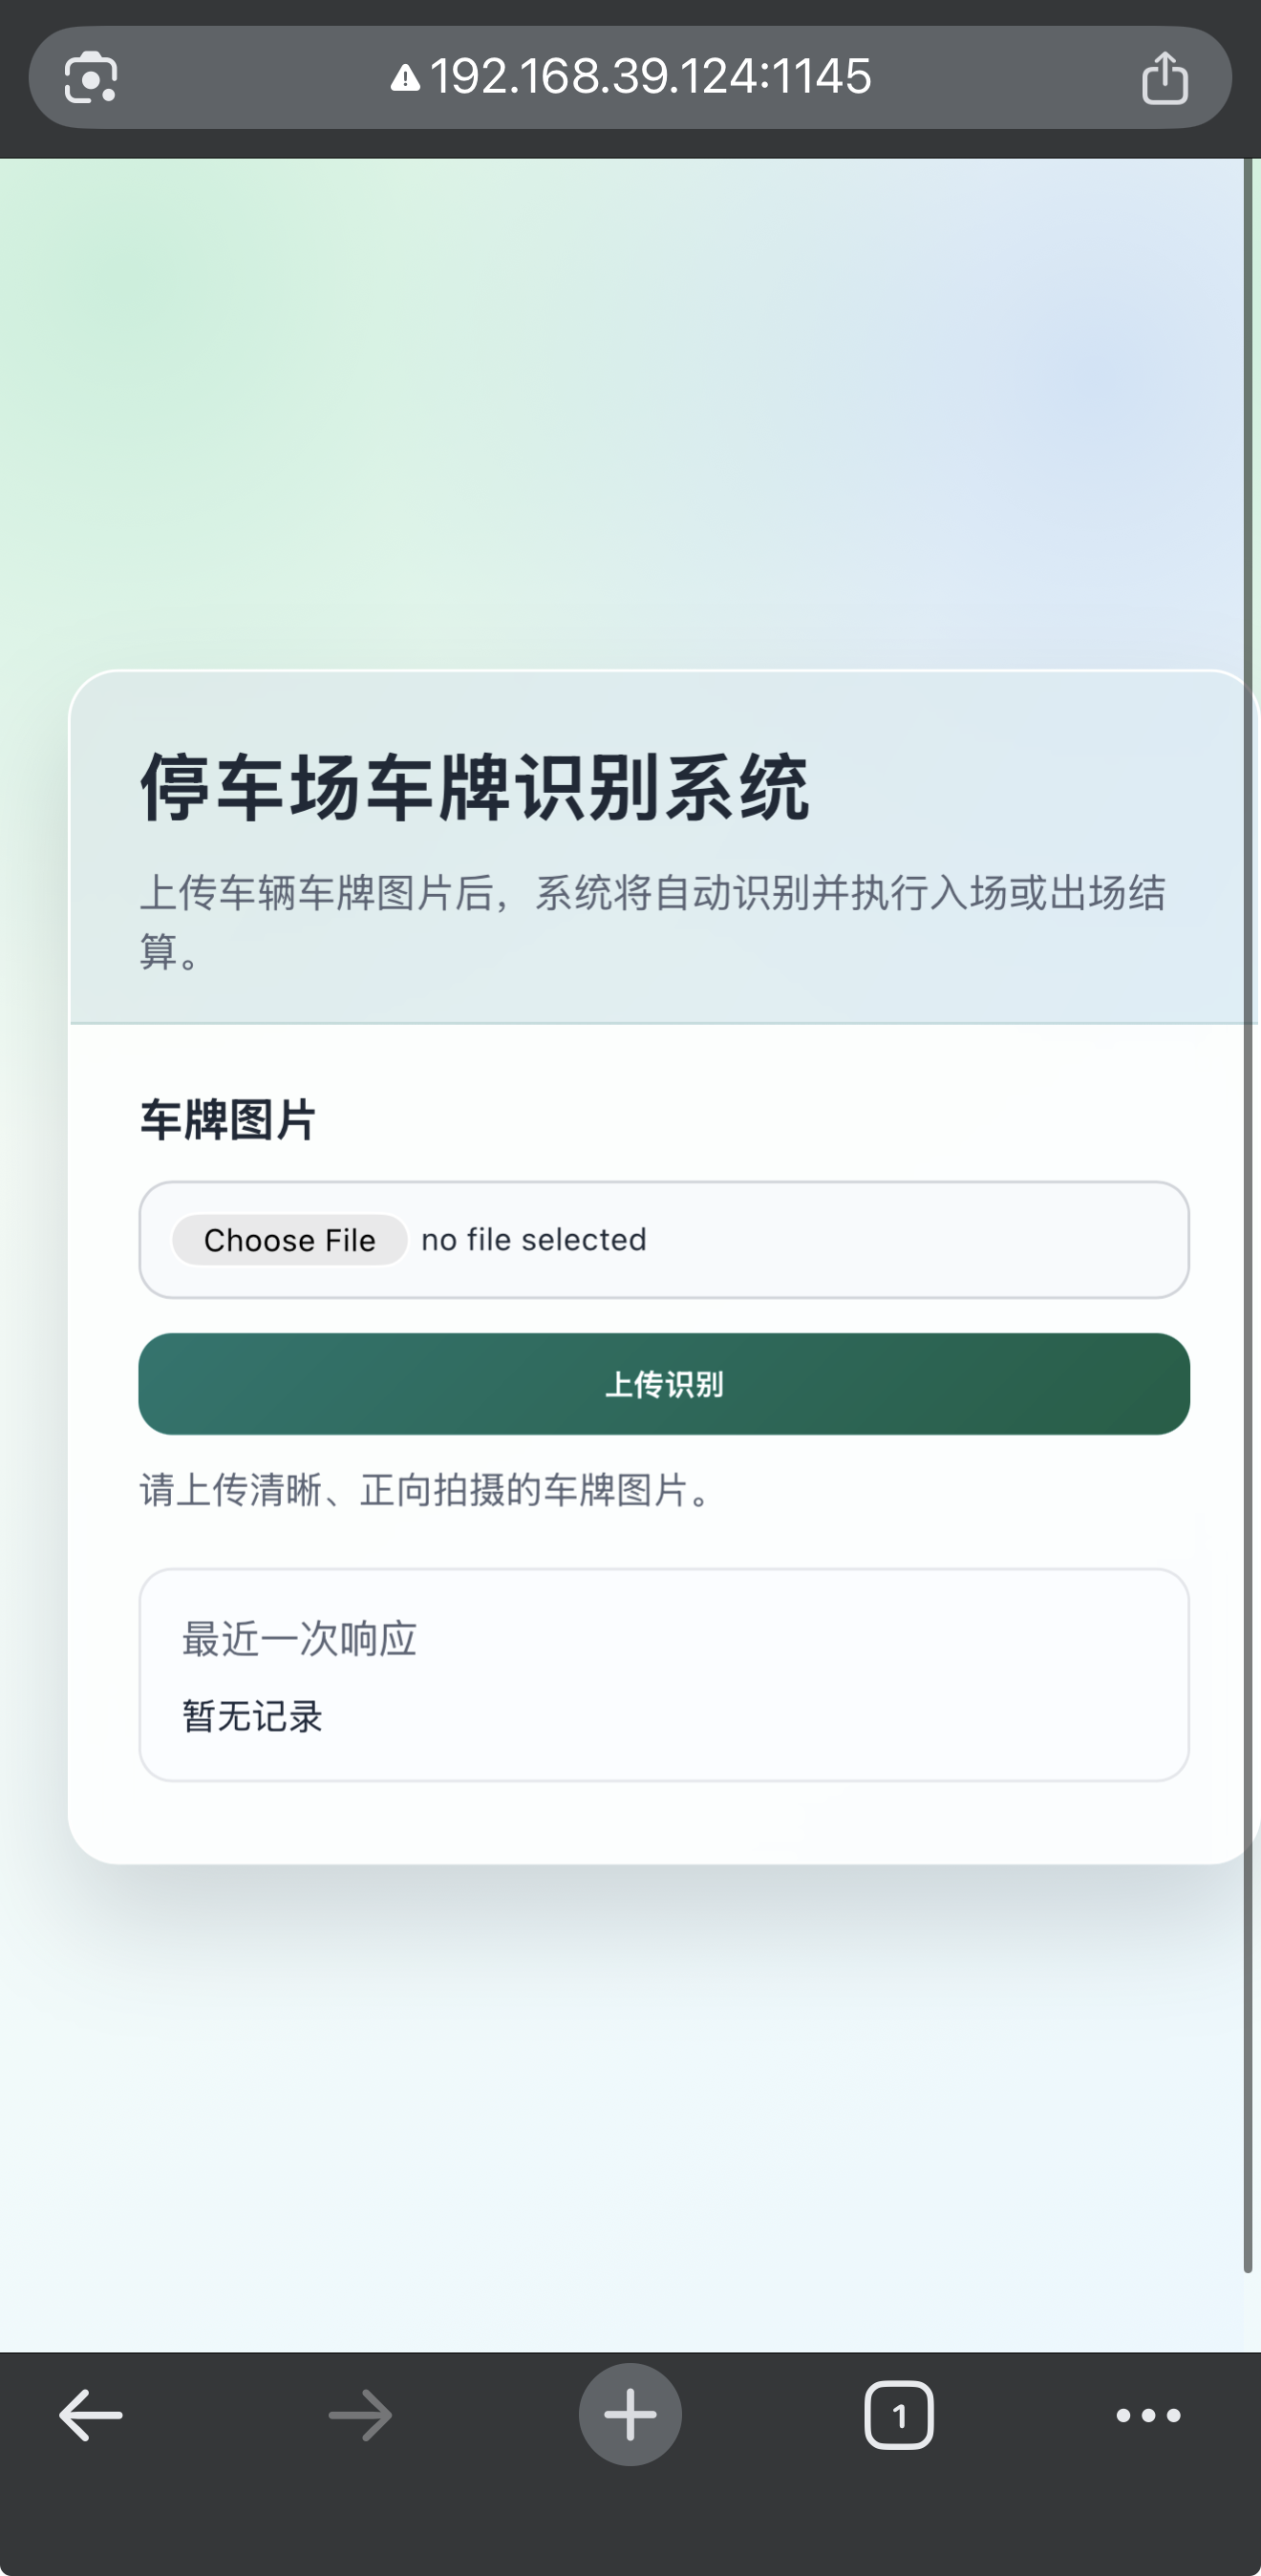
\includegraphics[width=0.44\textwidth]{images/webui.png}
  \caption{移动端首页UI}
  \label{fig:webui}
\end{figure}
\subsection*{附：新增UI与异常处理}
为提升操作清晰度与容错性，本次更新对前端和后端进行了两项重要补充：

\subsubsection*{（一）UI：入场/出场按钮分离}
页面顶部新增独立的“入场”和“出场”按钮，用户可在不改变下方主上传区的情况下直接选择操作类型。该交互把上传文件选择与业务意图显式分离，避免用户误操作导致错误计费。顶部控件与下方上传控件联动——在顶部选择文件会自动填入下方的上传输入框，点击顶部按钮即可触发带有 \texttt{channel} 参数的上传请求。图\ref{fig:new-ui} 展示了新增后的页面布局与按钮位置。

\begin{figure}[H]
  \centering
  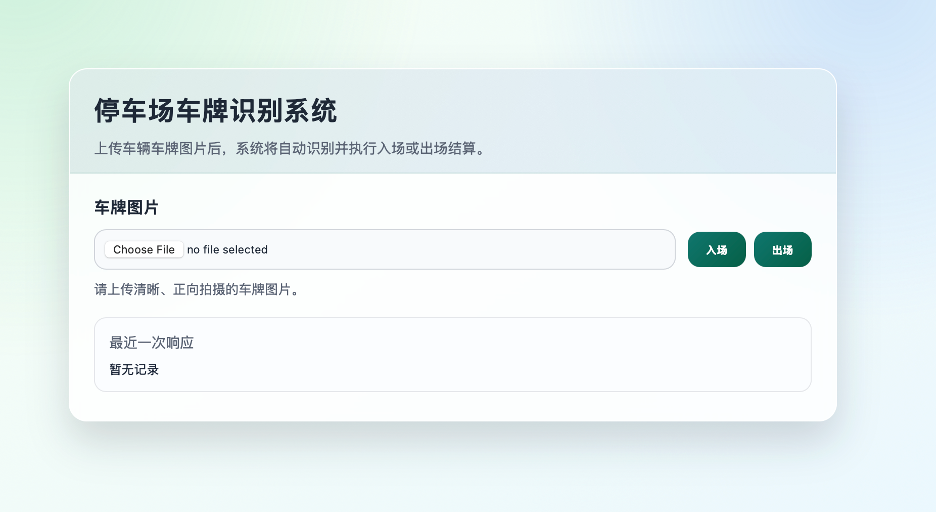
\includegraphics[width=0.7\textwidth]{images/new_ui.png}
  \caption{新增UI：顶部入场/出场按钮与主上传控件联动（示意）}
  \label{fig:New_web_ui}
\end{figure}

\subsubsection*{（二）异常处理：用户友好的错误提示与后端保护}
针对常见业务与识别异常，系统在服务端实现了统一错误码与可读提示，并由前端弹窗友好展示。新增的两类典型错误如下：

\begin{enumerate}
  \item \textbf{new\_error1：未入场先出场（exit\_before\_entry）}\\
    场景：用户上传一张车牌图片并选择“出场”，但数据库中不存在该车牌的在场记录。
    后端检测到此类请求会返回 HTTP 409，并给出错误码 \texttt{exit\_before\_entry} 及中文提示“未入场先出场：找不到在场记录”。前端在弹窗中展示该提示，避免用户误以为计费成功。图\ref{fig:new-error1-ui} 为前端提示示意，图\ref{fig:new-error1-term} 为后端日志/终端输出示意。

  \item \textbf{new\_error2：识别无效（ocr\_no\_plate）}\\
    场景：上传的图片无法识别出符合车牌规则的文本（例如模糊、角度不对或非车牌图片）。后端会返回 HTTP 422，并返回错误码 \texttt{ocr\_no\_plate} 以及提示“OCR识别失败或车牌不符合规则，请上传更清晰的正向车牌图片”。前端将该提示以弹窗形式告知用户，建议重拍或更换图片。图\ref{fig:new-error2-ui} 为前端提示示意，图\ref{fig:new-error2-term} 为后端日志/终端输出示意。
\end{enumerate}

\begin{figure}[H]
  \centering
  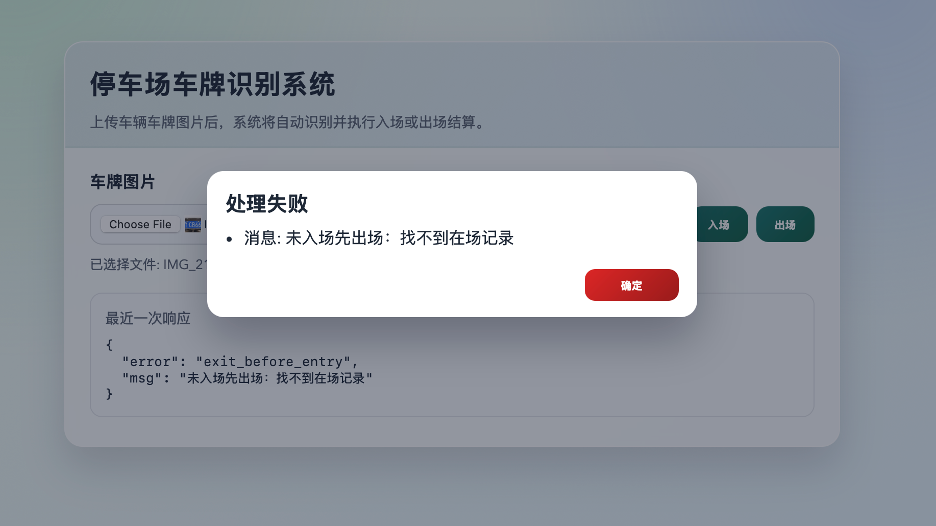
\includegraphics[width=0.44\textwidth]{images/New_error1.png}
  \caption{异常提示示例：未入场先出场（前端弹窗）}
  \label{fig:New_error1}
\end{figure}

\begin{figure}[H]
  \centering
  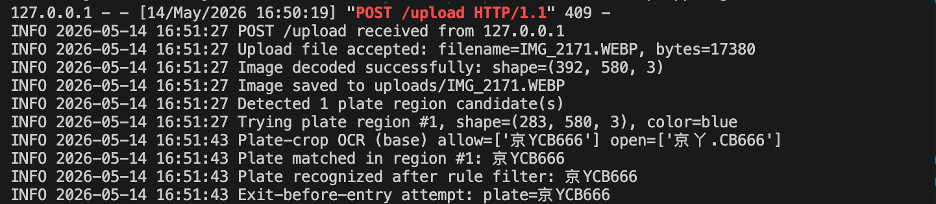
\includegraphics[width=0.95\textwidth]{images/New_error1_terminal.png}
  \caption{终端日志（示意）：未入场先出场被拦截并返回 409}
  \label{fig:New_error1_terminal}
\end{figure}

\begin{figure}[H]
  \centering
  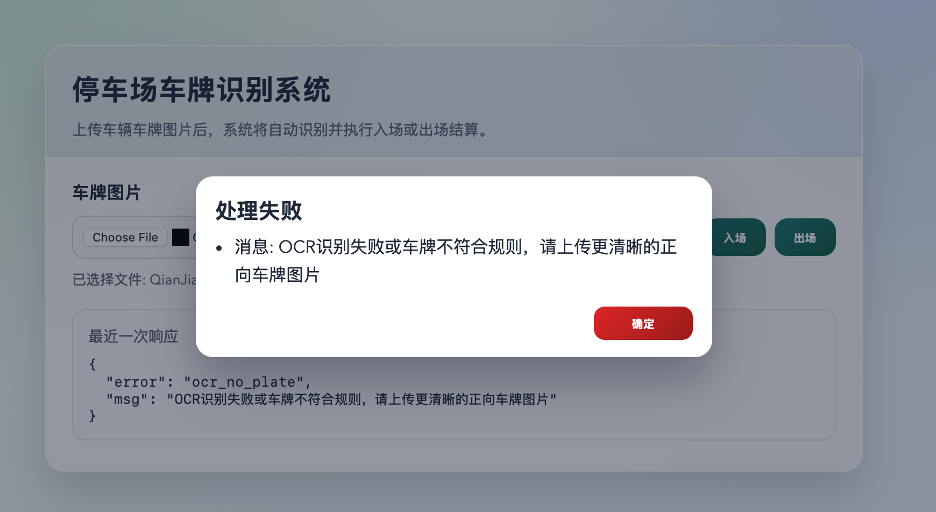
\includegraphics[width=0.44\textwidth]{images/New_error2.png}
  \caption{异常提示示例：OCR无法匹配车牌（前端弹窗）}
  \label{fig:New_error2}
\end{figure}

\begin{figure}[H]
  \centering
  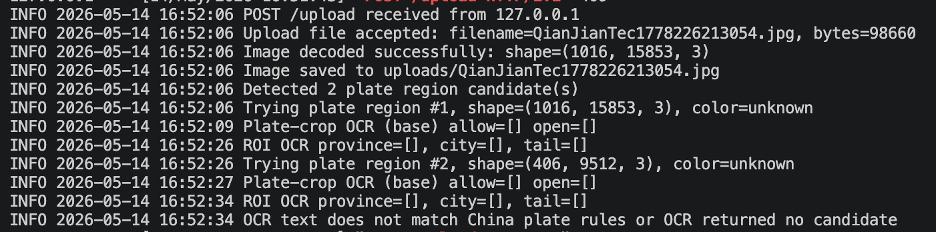
\includegraphics[width=0.95\textwidth]{images/New_error2_terminal.png}
  \caption{终端日志（示意）：OCR初始化/识别失败返回 422 或 502，便于定位问题}
  \label{fig:New_error2_terminal}
\end{figure}

以上异常处理在代码中使用明确的错误码与 HTTP 状态码进行区分（见 \texttt{app.py} 中的返回分支），这既便于前端按类型展示不同的交互，也方便自动化测试断言错误类型，提升系统可维护性。

\subsection*{1. 测试一：样本1（苏B92912）入场与出场}
\textbf{测试目标：}验证规则增强OCR在“省份汉字+城市字母+数字后缀”典型蓝牌场景下的稳定性。

\textbf{入场过程与结果：}图\ref{fig:t1-entry-server}显示服务端检测到候选区域后，经过OCR与规则筛选得到\texttt{苏B92912}，并写入入场记录；图\ref{fig:t1-entry-ui}显示前端弹窗反馈“入场成功”。

\begin{figure}[H]
  \centering
  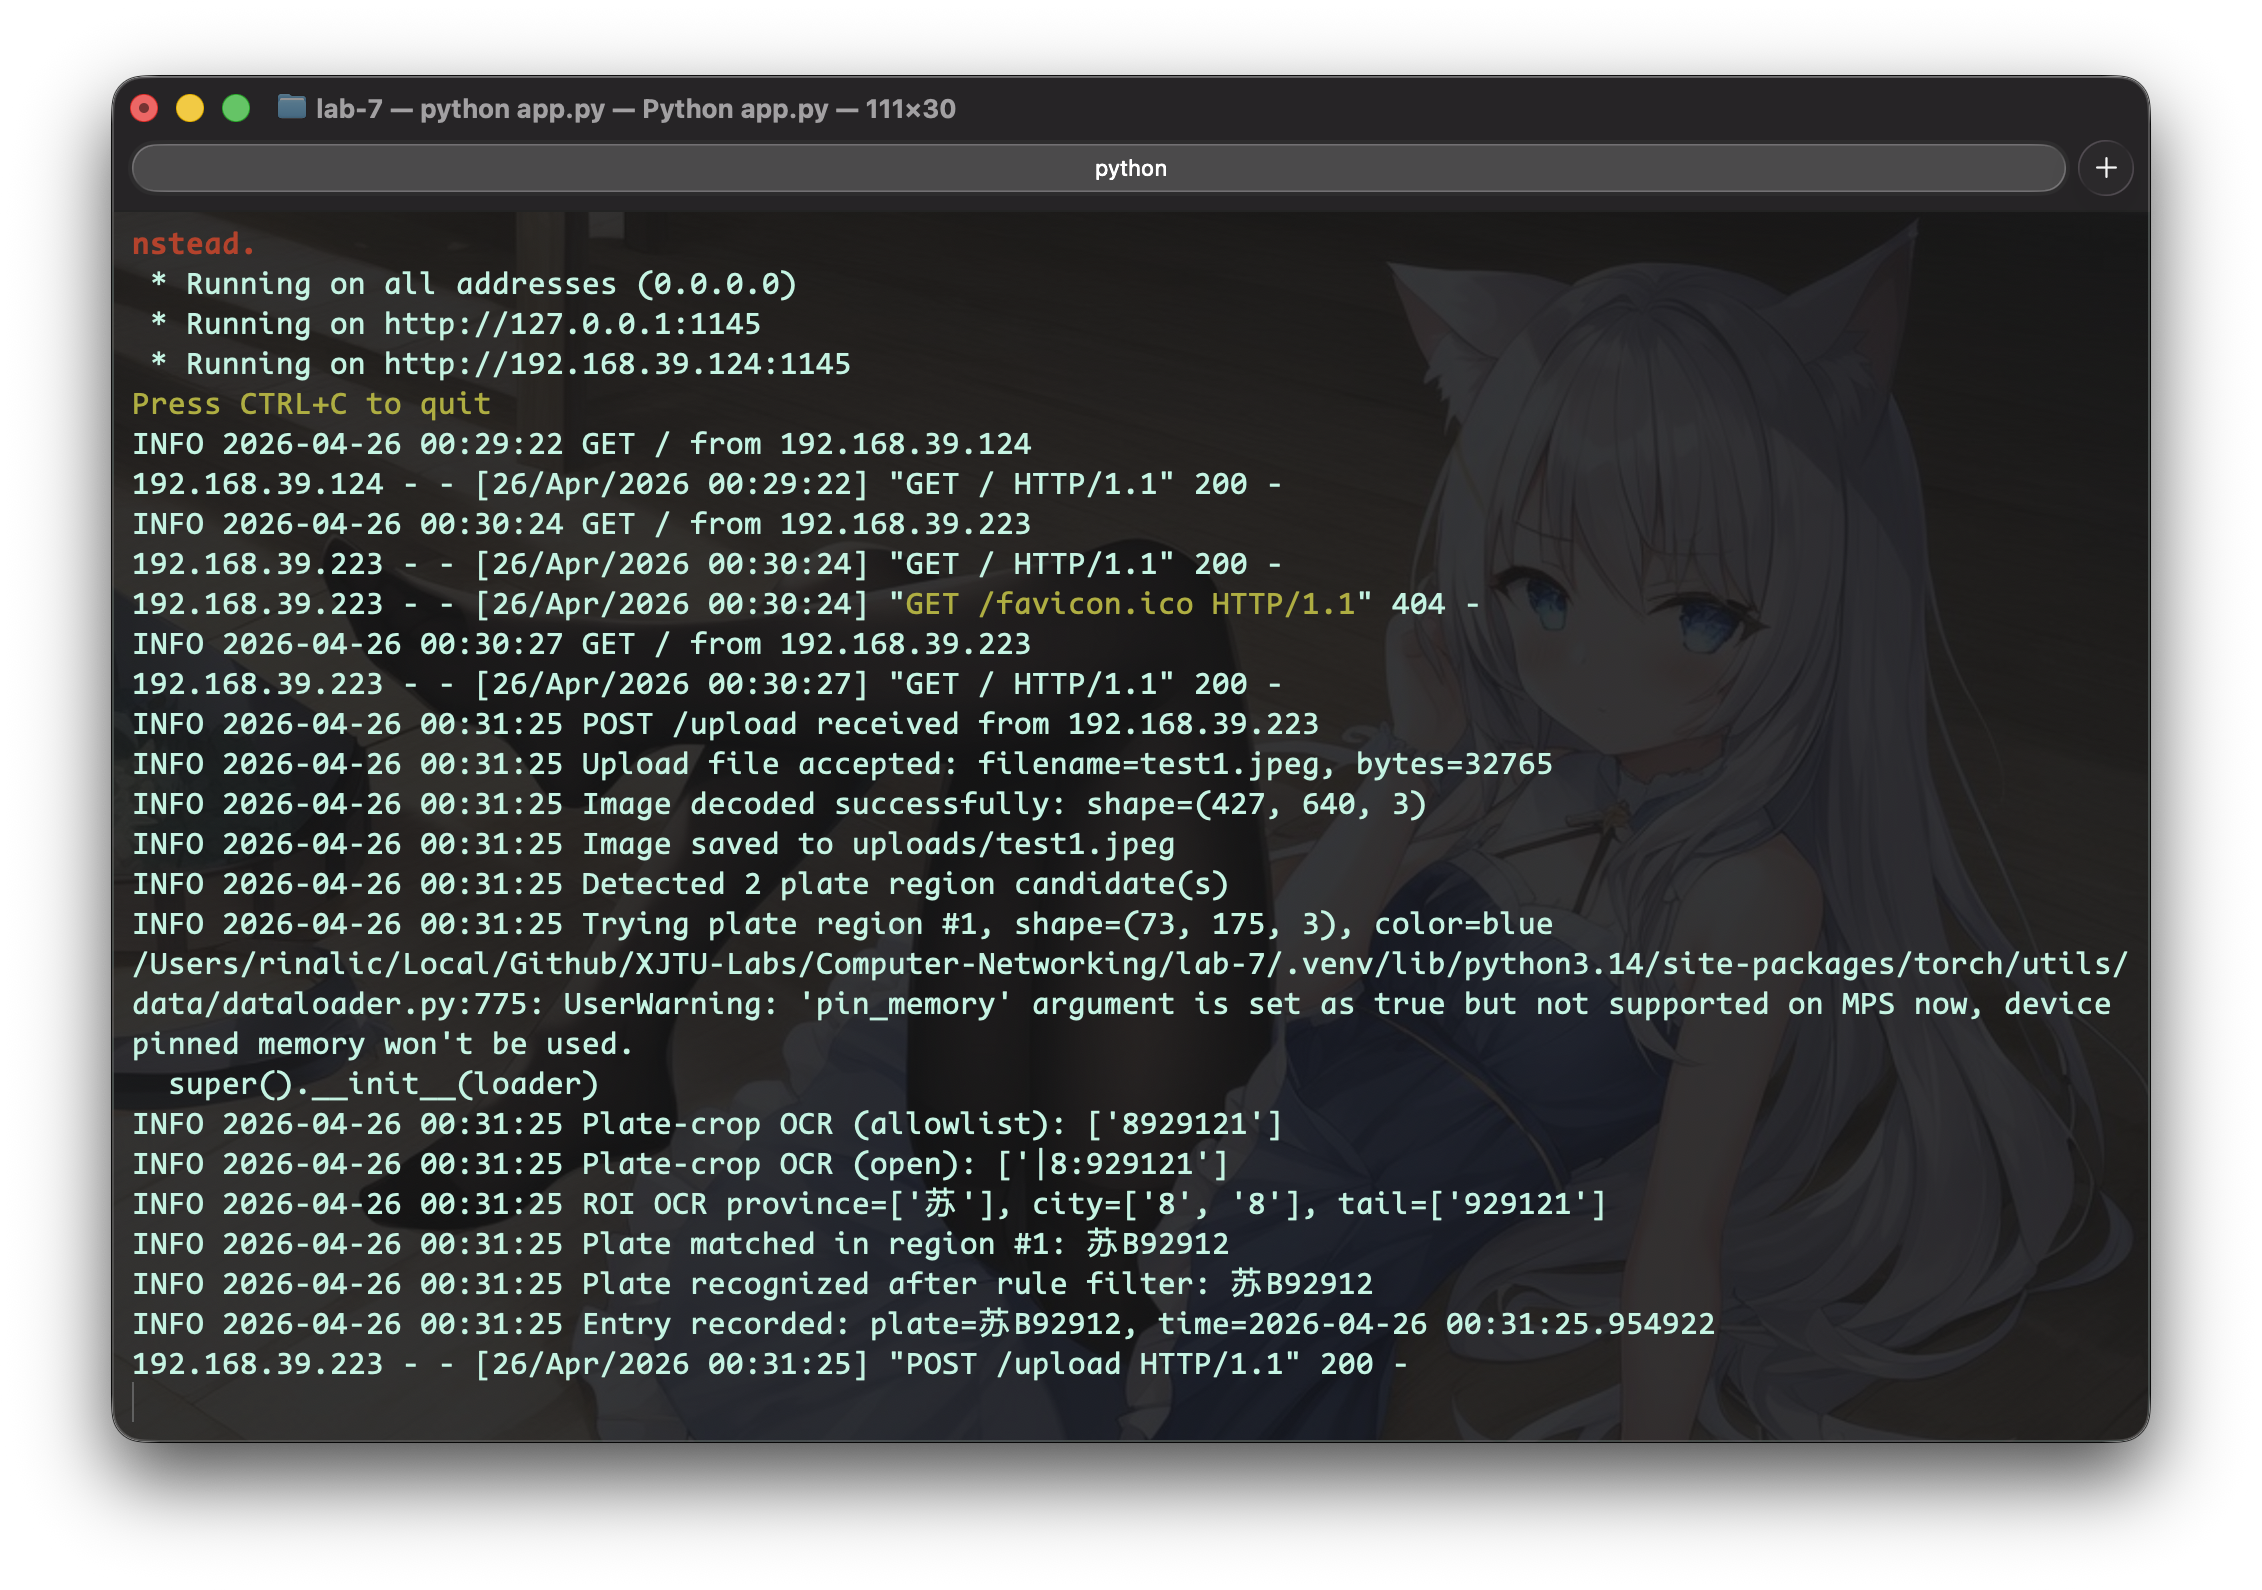
\includegraphics[width=0.95\textwidth]{images/test_1_entry_server.png}
  \caption{测试一入场：服务端日志（识别并写入在场记录）}
  \label{fig:t1-entry-server}
\end{figure}

\begin{figure}[H]
  \centering
  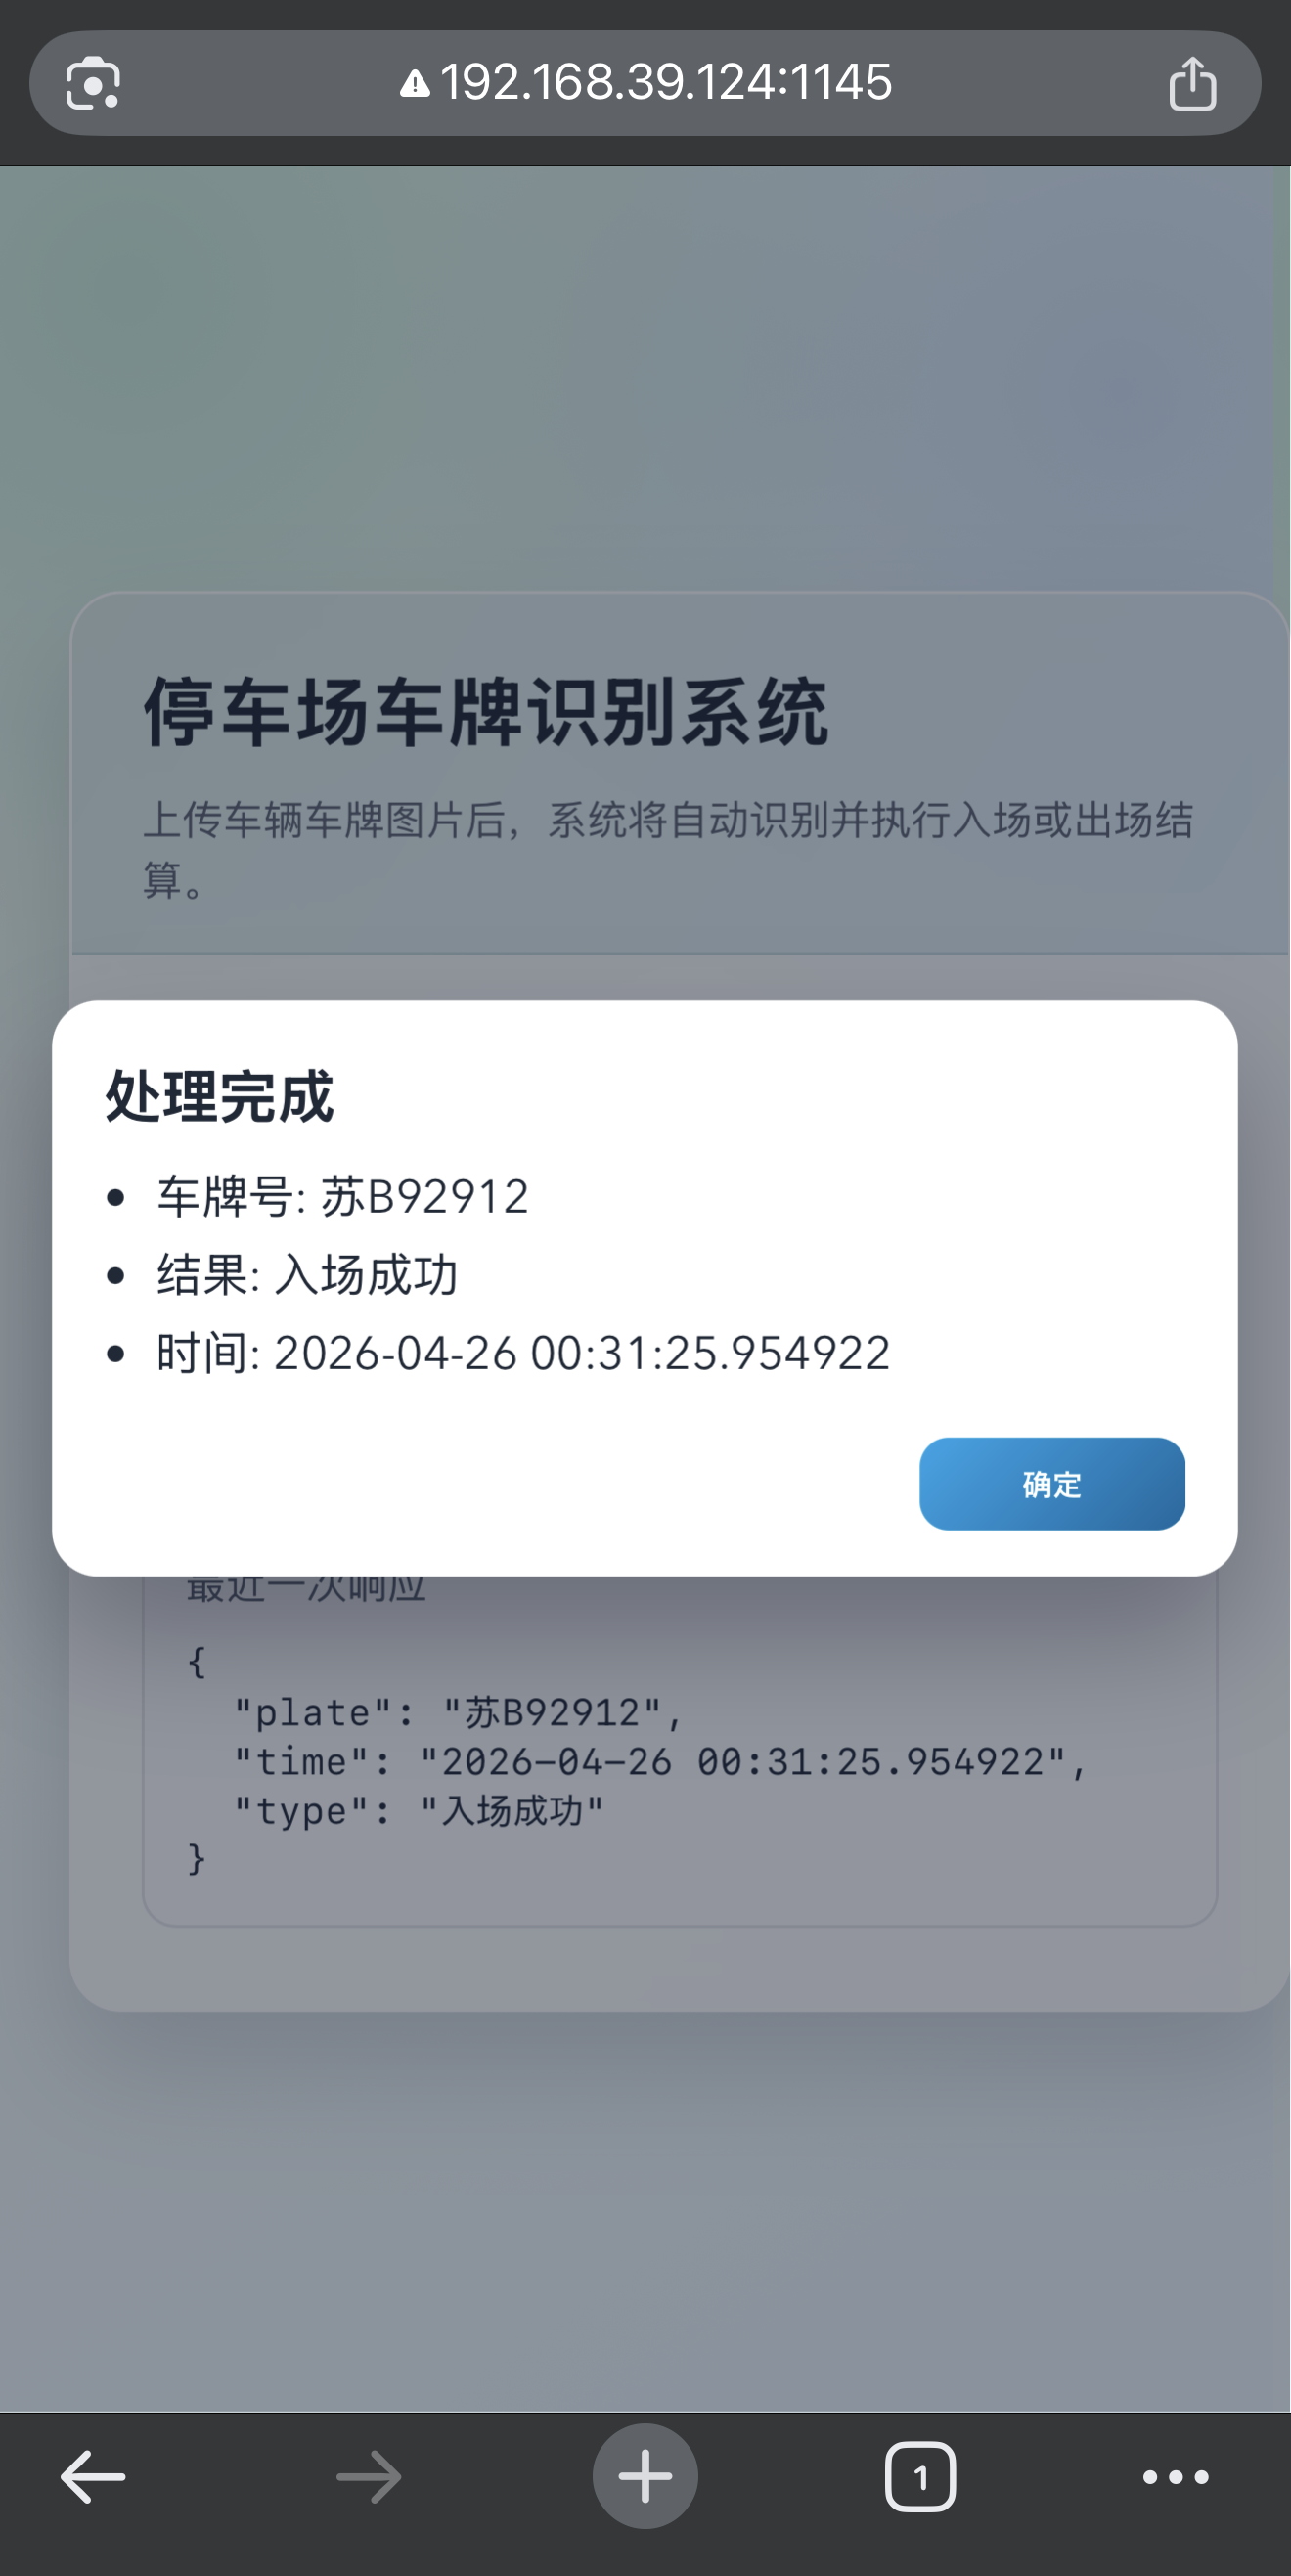
\includegraphics[width=0.44\textwidth]{images/test_1_entry_webui.png}
  \caption{测试一入场：前端弹窗结果}
  \label{fig:t1-entry-ui}
\end{figure}

\textbf{出场过程与结果：}图\ref{fig:t1-exit-server}显示再次上传同一车牌后，系统匹配在场记录并完成出场结算，返回费用0.34元；图\ref{fig:t1-exit-ui}显示前端准确展示费用字段。

\begin{figure}[H]
  \centering
  \includegraphics[width=0.95\textwidth]{images/test_1_exit_server.png}
  \caption{测试一出场：服务端日志（匹配在场记录并计费）}
  \label{fig:t1-exit-server}
\end{figure}

\begin{figure}[H]
  \centering
  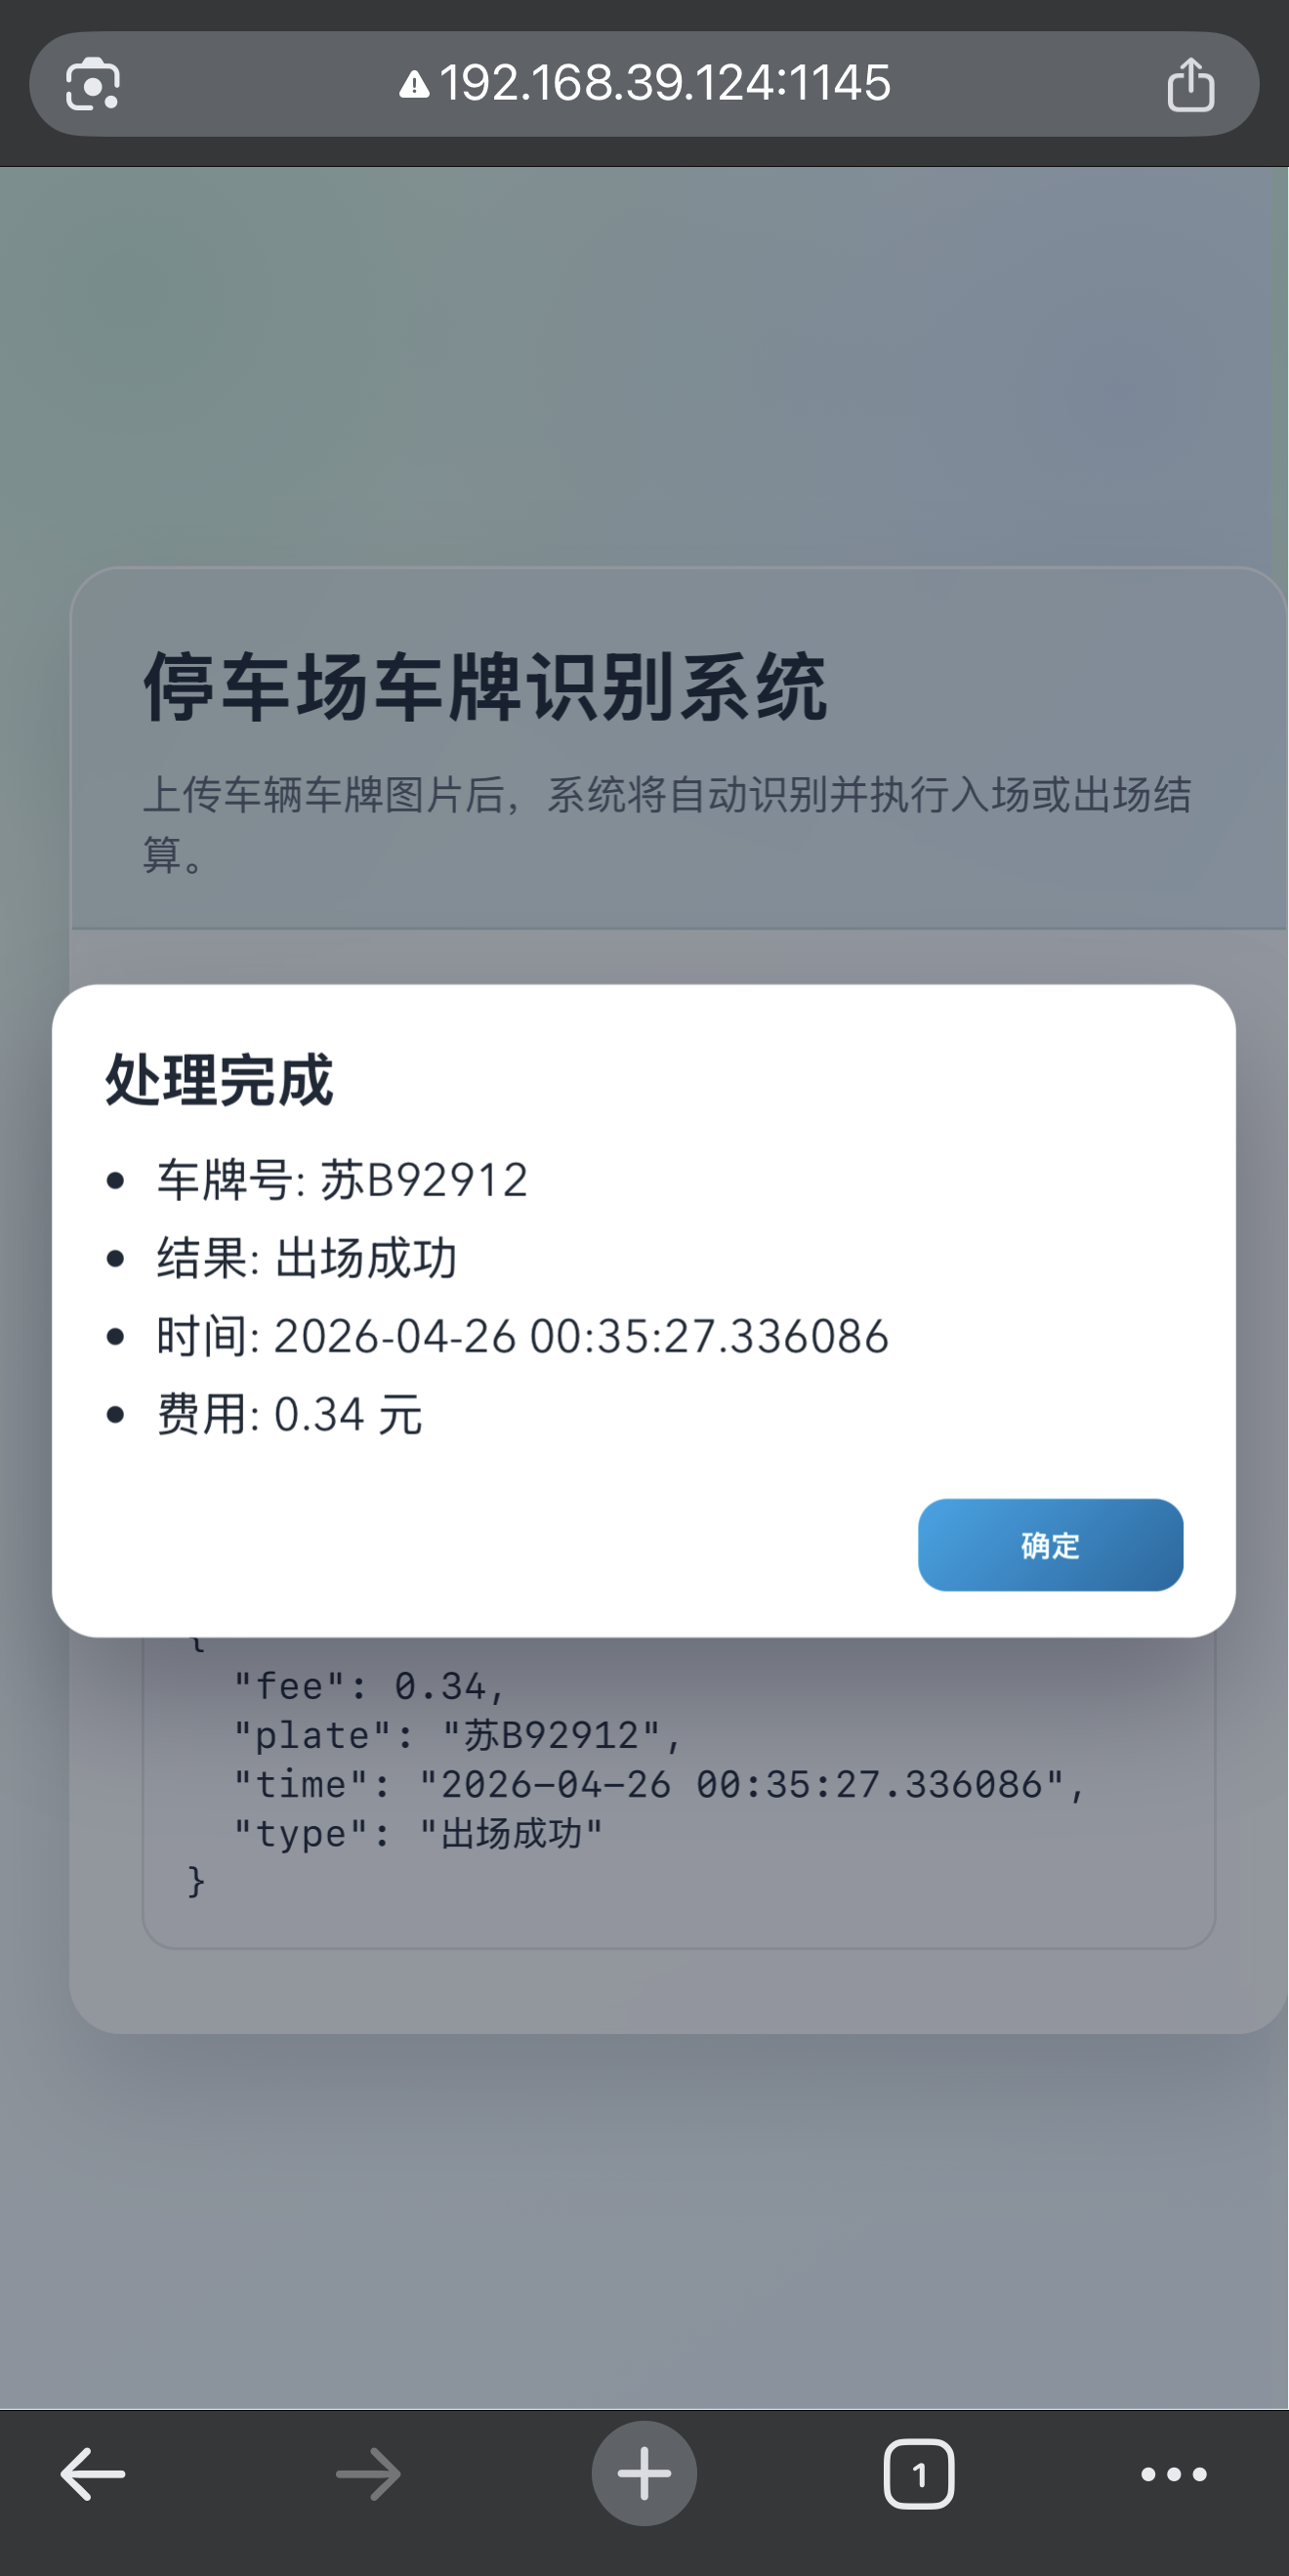
\includegraphics[width=0.44\textwidth]{images/test_1_exit_webui.png}
  \caption{测试一出场：前端弹窗结果（含费用）}
  \label{fig:t1-exit-ui}
\end{figure}

\textbf{分析：}测试一验证了规则增强策略对“\texttt{B/8}混淆”问题的修正能力。日志中的中间结果可以看到城市位OCR曾出现数字，但最终经过映射和打分后得到正确城市字母，说明改进逻辑有效。

\subsection*{2. 测试二：样本2（京YCB666）入场与出场}
\textbf{测试目标：}验证包含字母+字母+数字混合后缀的蓝牌样本识别能力。

\textbf{入场过程与结果：}图\ref{fig:t2-entry-server}显示系统在首个候选区域即识别到\texttt{京YCB666}并写入入场；图\ref{fig:t2-entry-ui}显示前端弹窗与日志一致。

\begin{figure}[H]
  \centering
  \includegraphics[width=0.95\textwidth]{images/test_2_entry_server.png}
  \caption{测试二入场：服务端日志（字母数字混合后缀识别）}
  \label{fig:t2-entry-server}
\end{figure}

\begin{figure}[H]
  \centering
  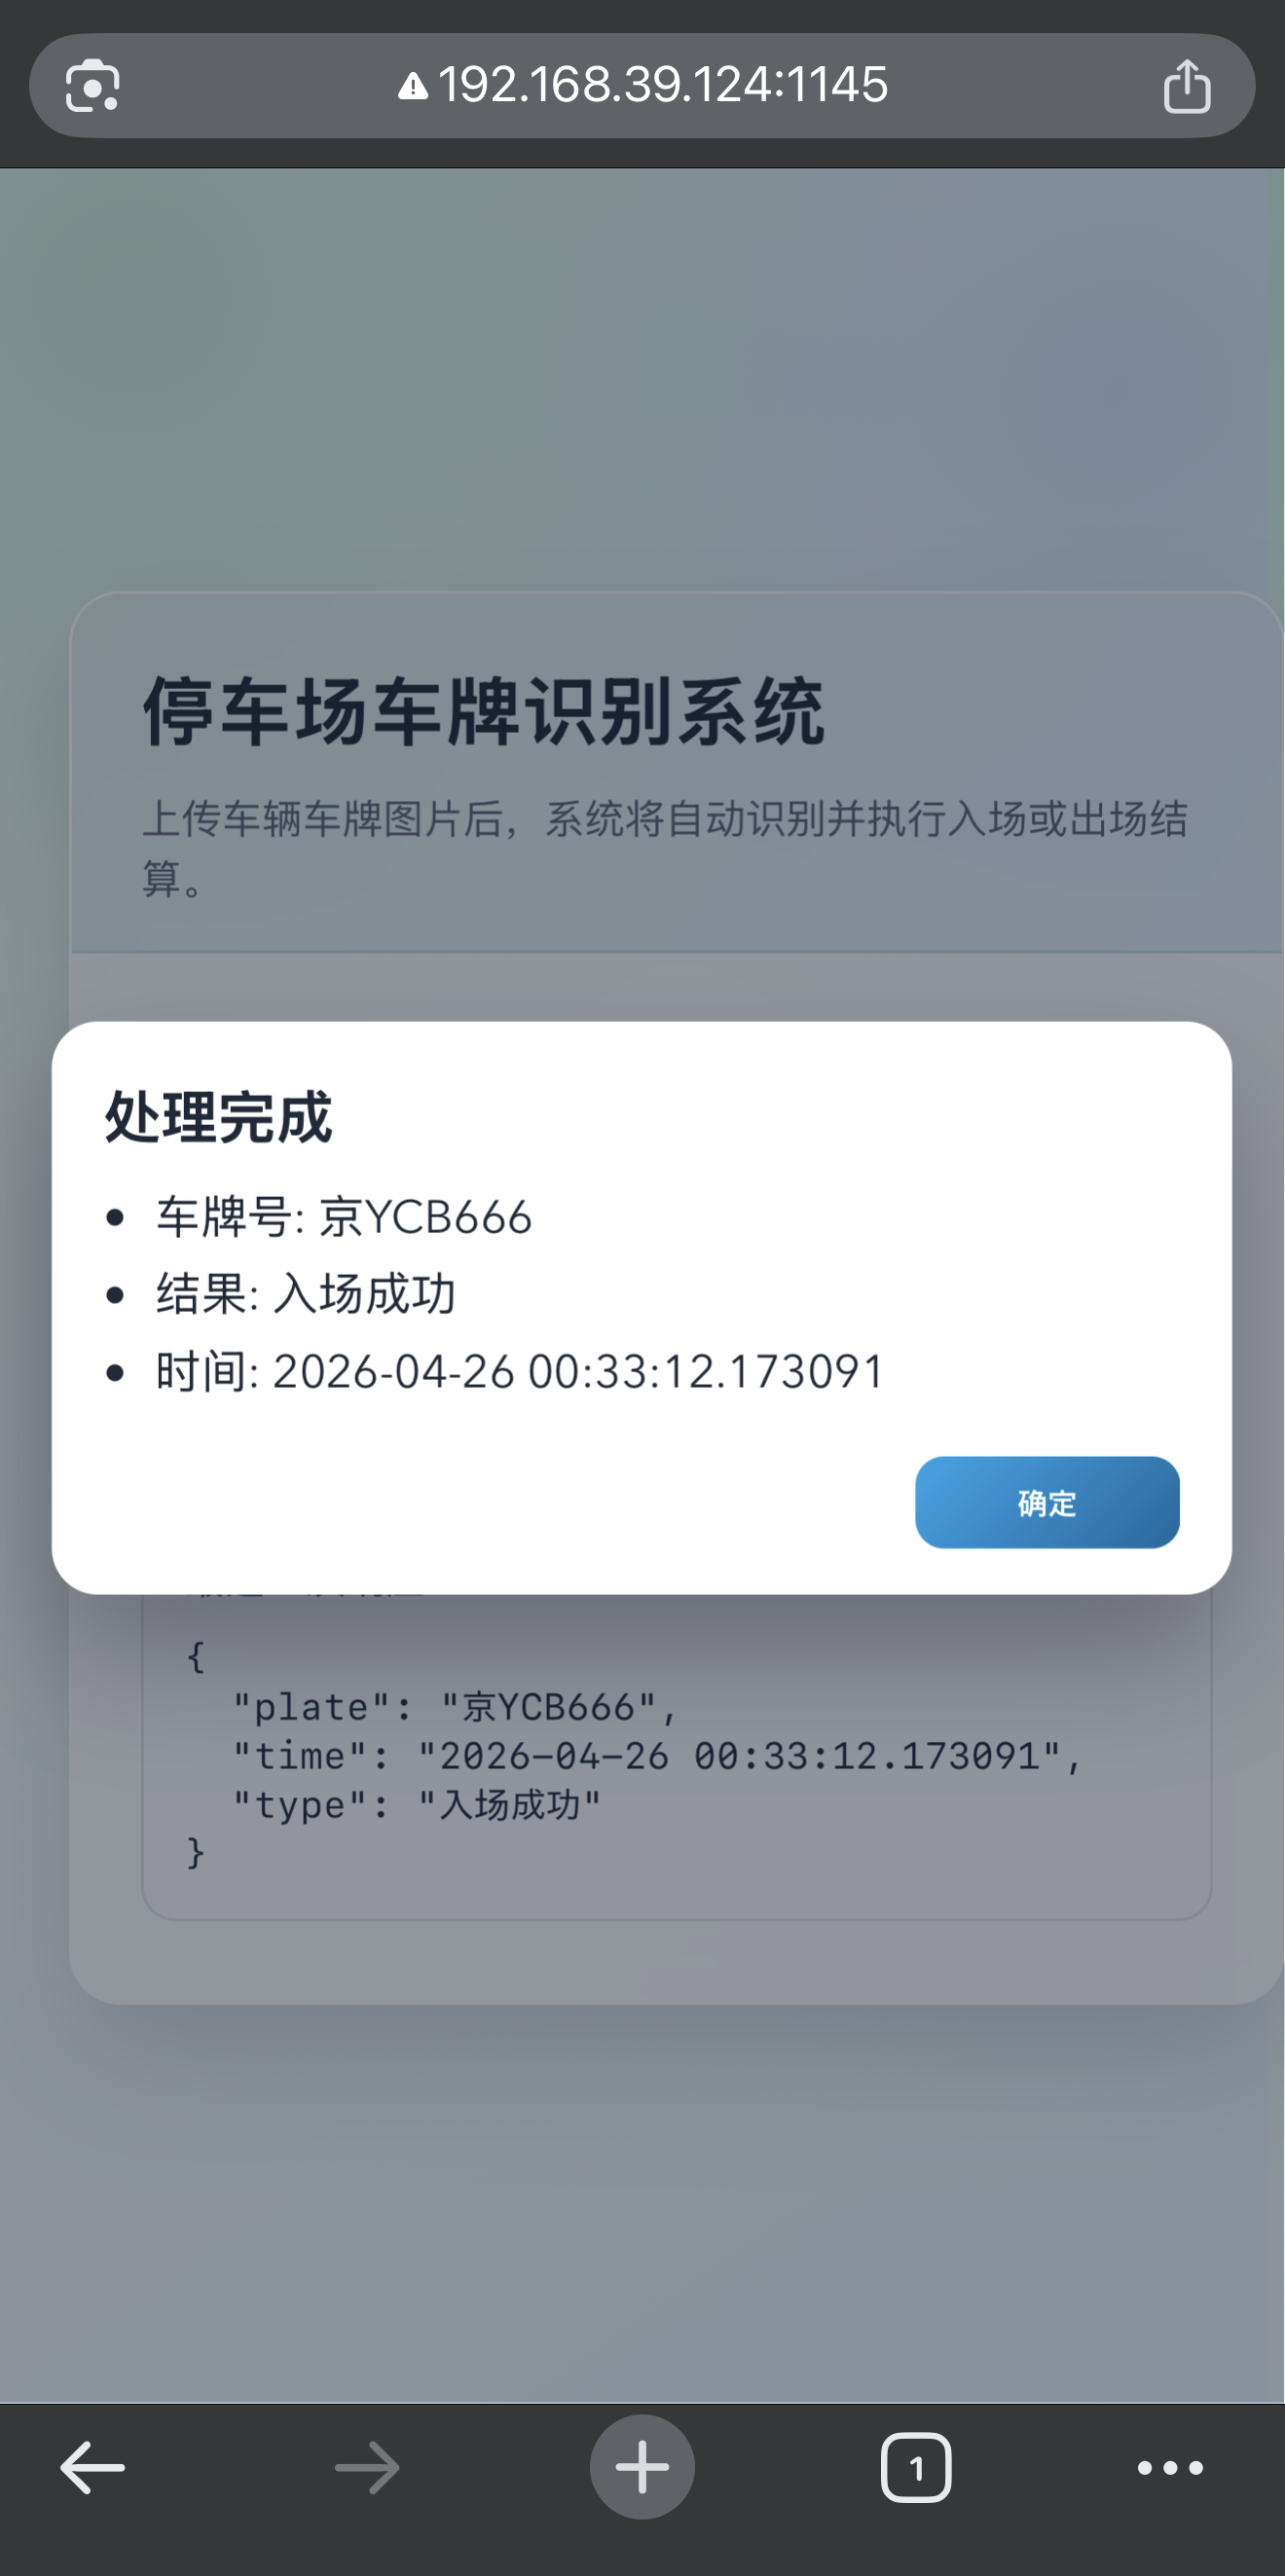
\includegraphics[width=0.44\textwidth]{images/test_2_entry_webui.png}
  \caption{测试二入场：前端弹窗结果}
  \label{fig:t2-entry-ui}
\end{figure}

\textbf{出场过程与结果：}图\ref{fig:t2-exit-server}显示系统能够从数据库中查找到在场记录并完成费用计算，金额为0.27元；图\ref{fig:t2-exit-ui}给出一致反馈。

\begin{figure}[H]
  \centering
  \includegraphics[width=0.95\textwidth]{images/test_2_exit_server.png}
  \caption{测试二出场：服务端日志（正常计费）}
  \label{fig:t2-exit-server}
\end{figure}

\begin{figure}[H]
  \centering
  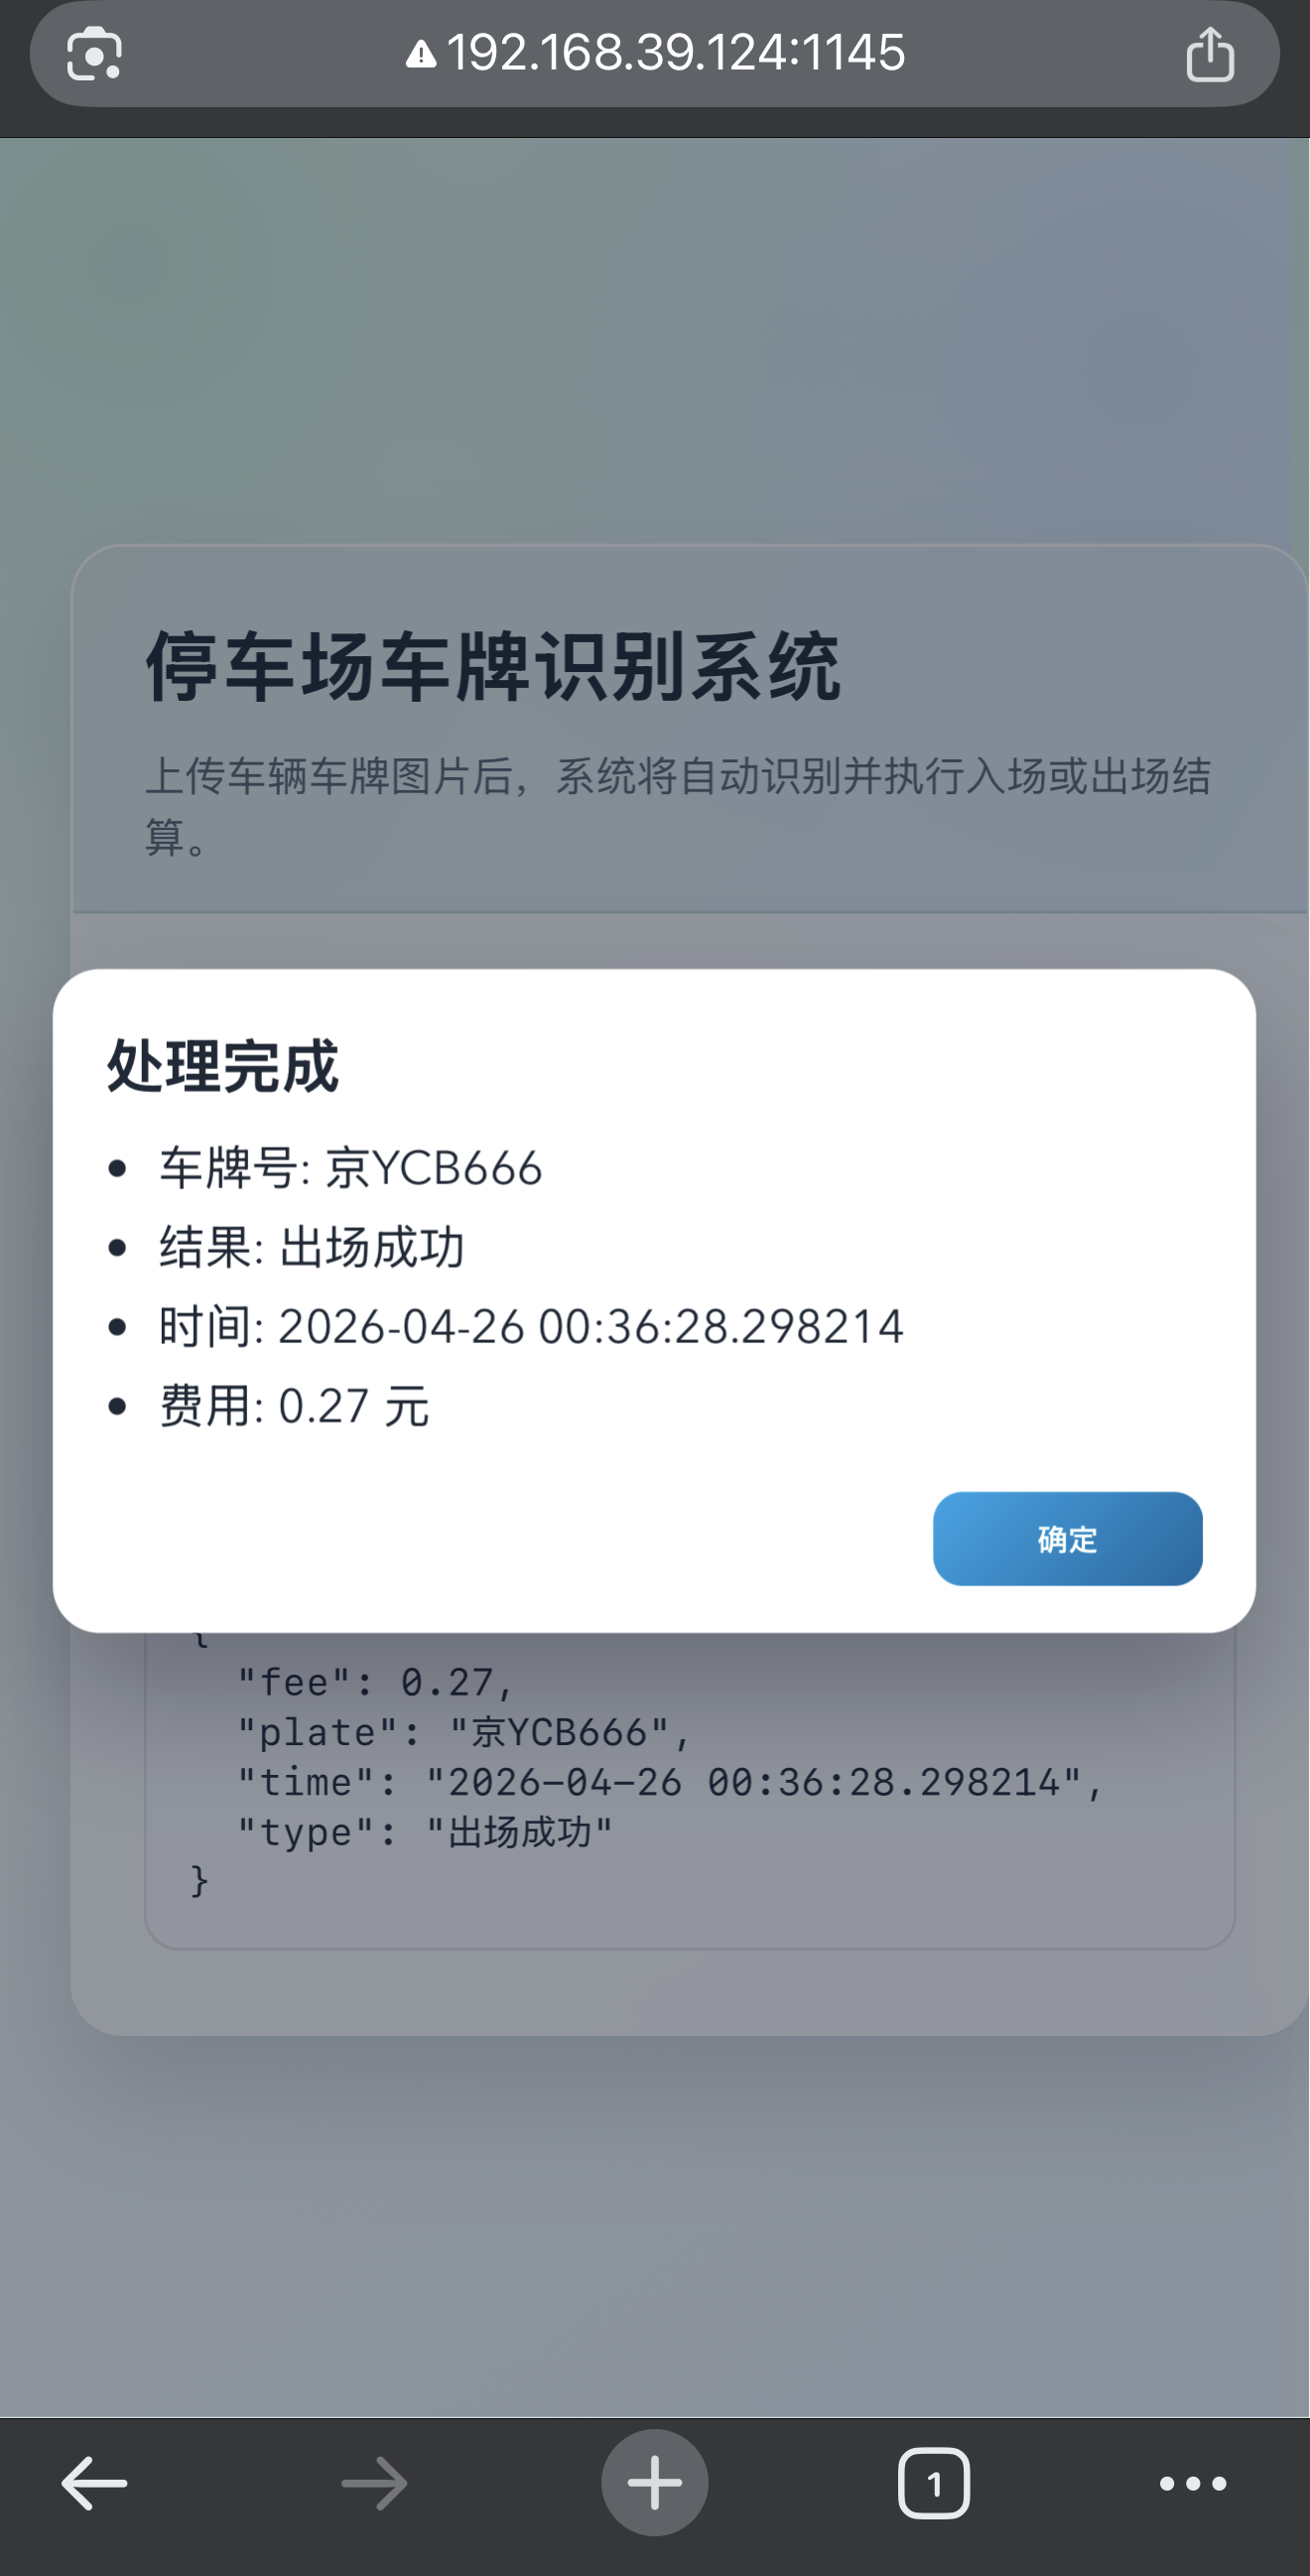
\includegraphics[width=0.44\textwidth]{images/test_2_exit_webui.png}
  \caption{测试二出场：前端弹窗结果（含费用）}
  \label{fig:t2-exit-ui}
\end{figure}

\textbf{分析：}测试二说明系统不仅能识别“纯数字尾号”类型，也能正确处理字母与数字混合尾号。该能力来自于后缀允许字符集\texttt{[A-Z0-9]}和长度规则共同约束。

\subsection*{3. 测试三：样本3（京A00001）入场与出场}
\textbf{测试目标：}验证在大图、多候选区域情况下的鲁棒性与回退机制。

\textbf{入场过程与结果：}图\ref{fig:t3-entry-server}显示此样本分辨率较高，系统检测到5个候选区域，首候选失败后自动尝试次候选并成功识别\texttt{京A00001}；图\ref{fig:t3-entry-ui}显示前端反馈入场成功。

\begin{figure}[H]
  \centering
  \includegraphics[width=0.95\textwidth]{images/test_3_entry_server.png}
  \caption{测试三入场：服务端日志（多候选回退后识别成功）}
  \label{fig:t3-entry-server}
\end{figure}

\begin{figure}[H]
  \centering
  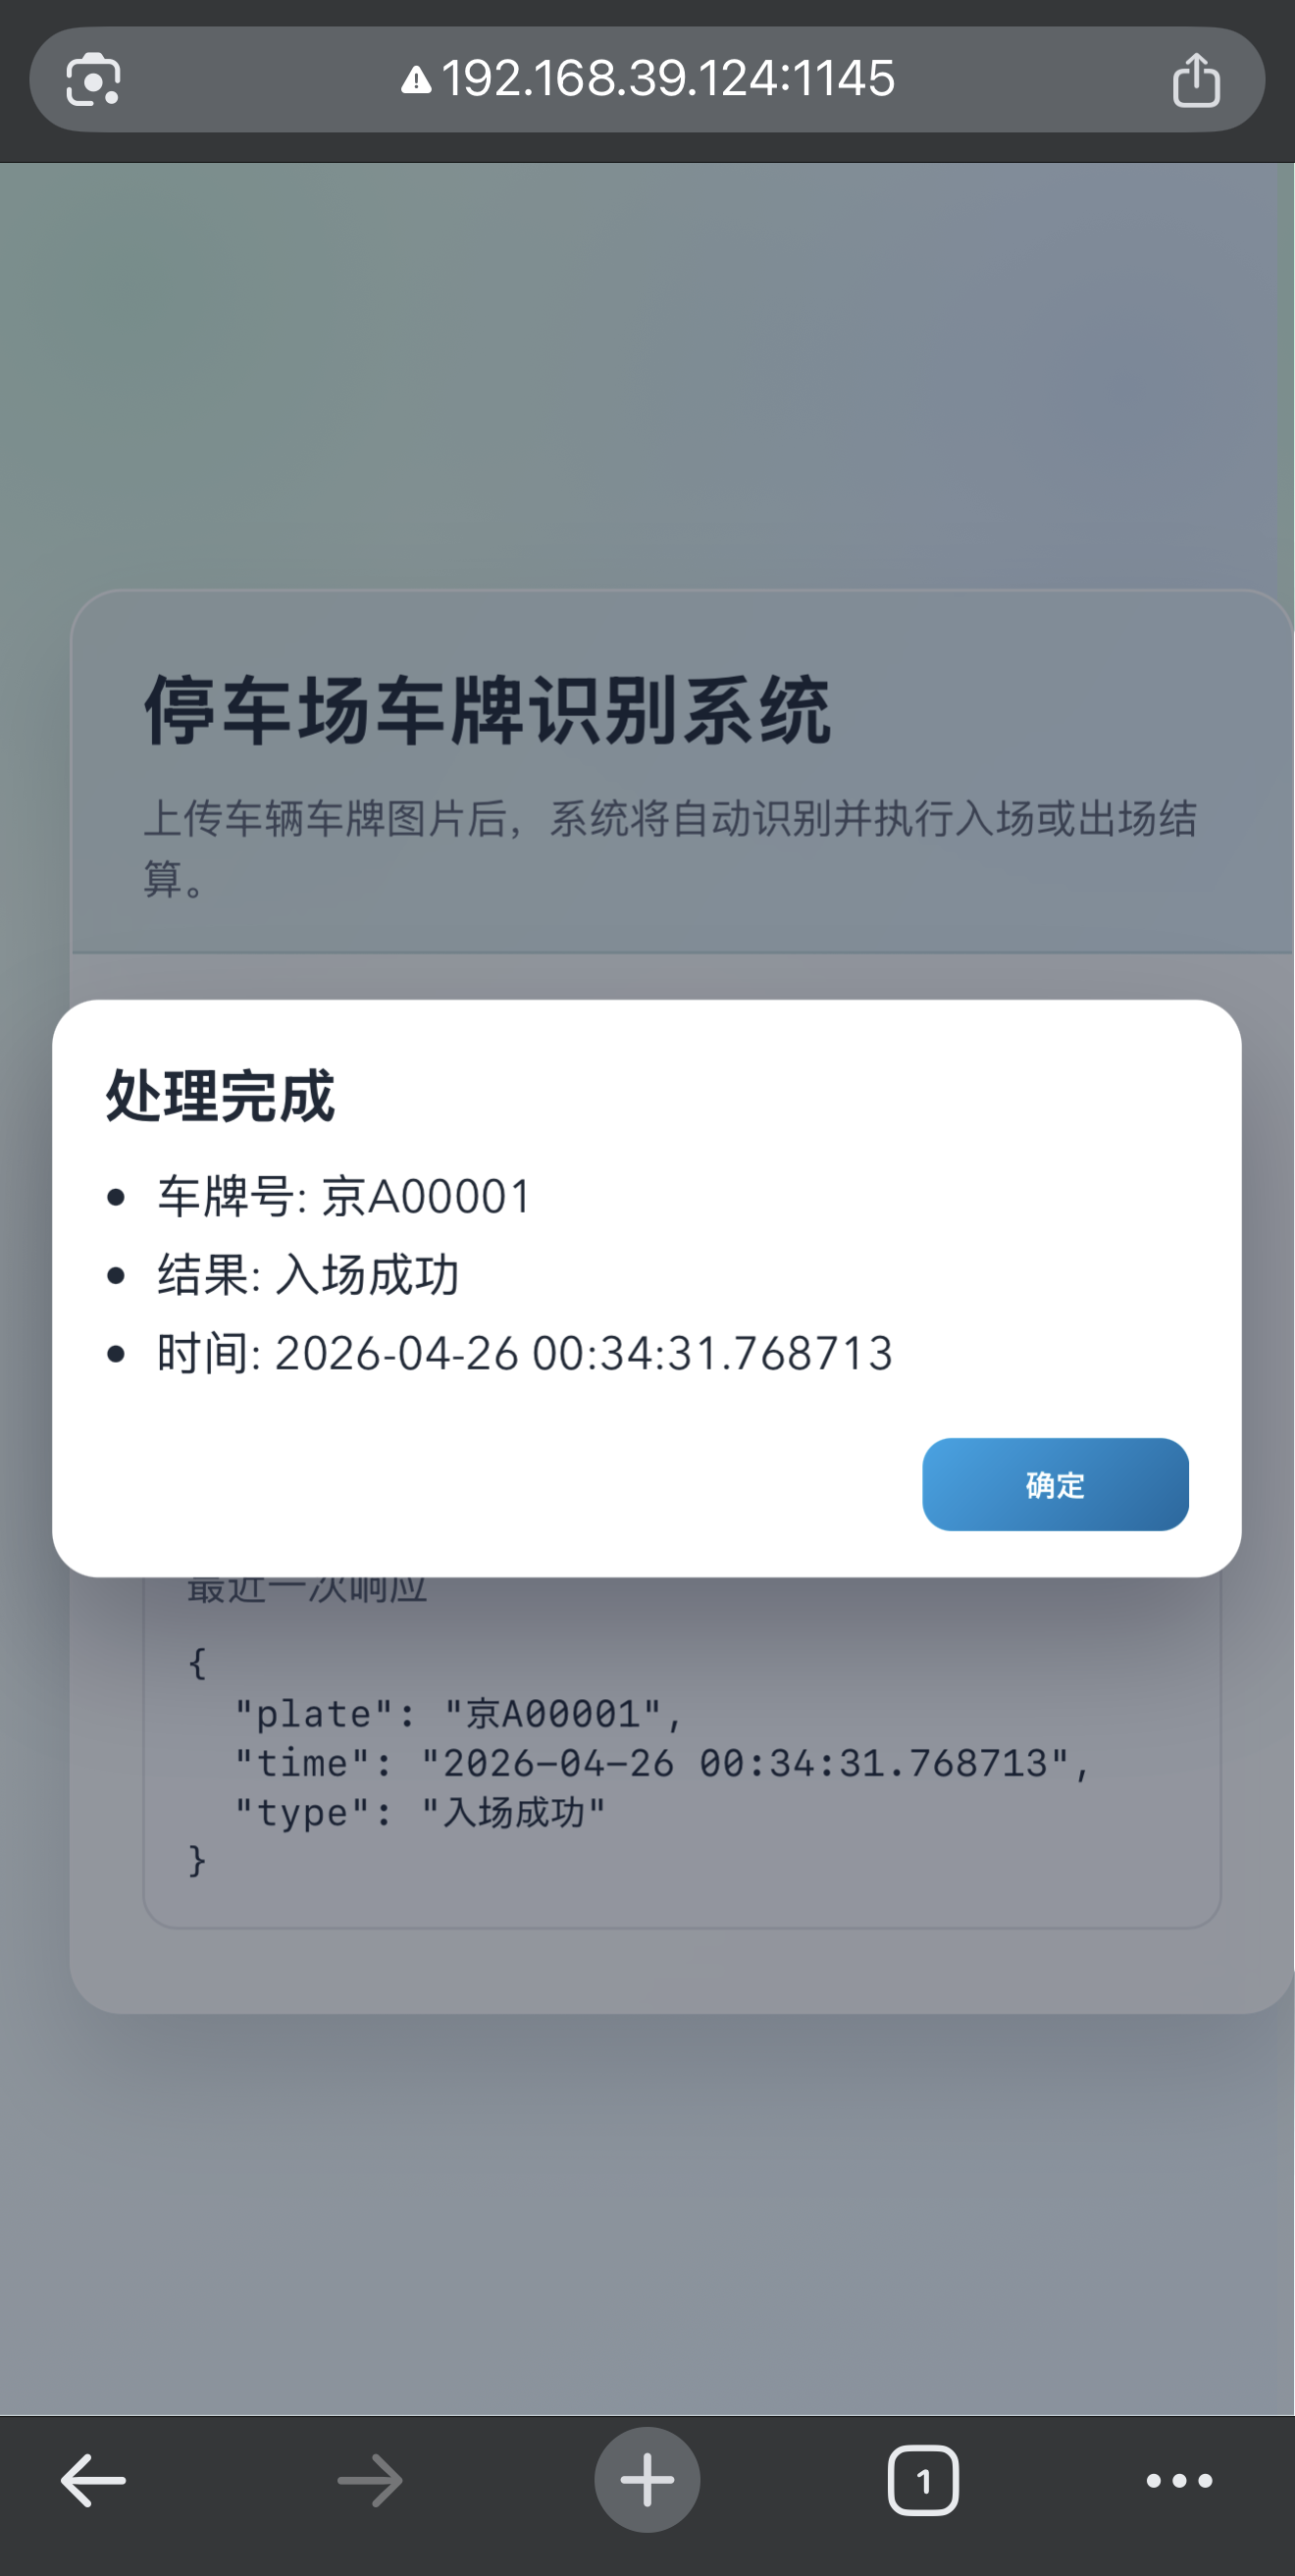
\includegraphics[width=0.44\textwidth]{images/test_3_entry_webui.png}
  \caption{测试三入场：前端弹窗结果}
  \label{fig:t3-entry-ui}
\end{figure}

\textbf{出场过程与结果：}图\ref{fig:t3-exit-server}可见系统再次走多候选流程并最终识别成功，完成出场计费0.28元；图\ref{fig:t3-exit-ui}显示结果一致。

\begin{figure}[H]
  \centering
  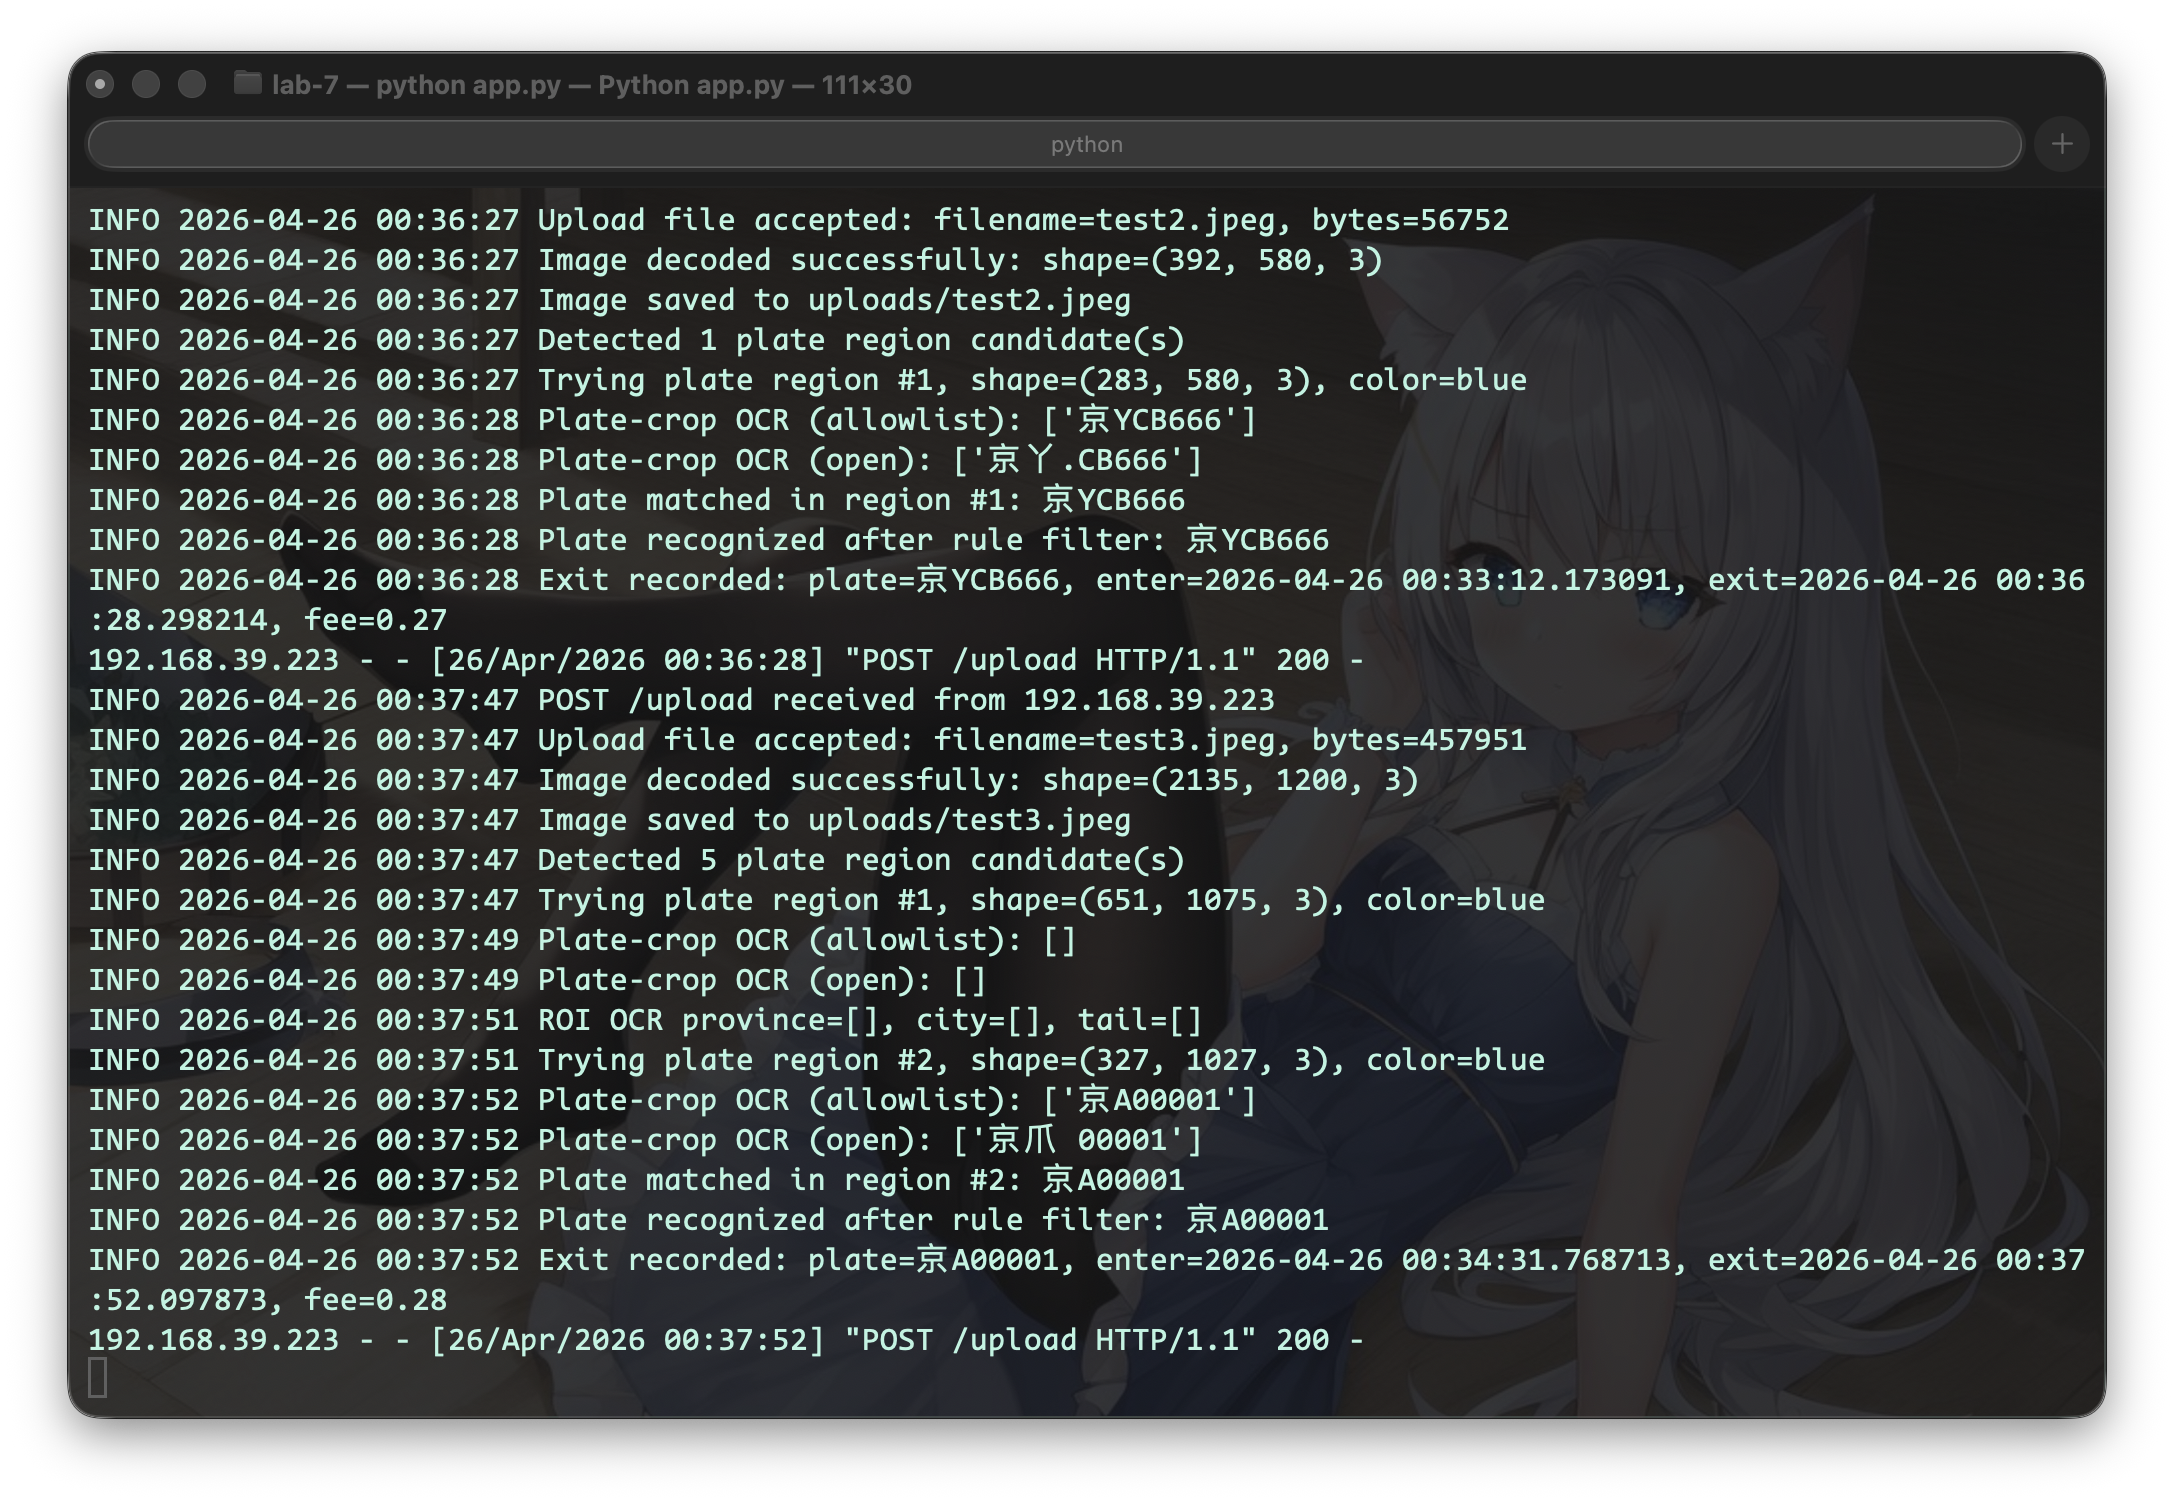
\includegraphics[width=0.95\textwidth]{images/test_3_exit_server.png}
  \caption{测试三出场：服务端日志（多候选+计费）}
  \label{fig:t3-exit-server}
\end{figure}

\begin{figure}[H]
  \centering
  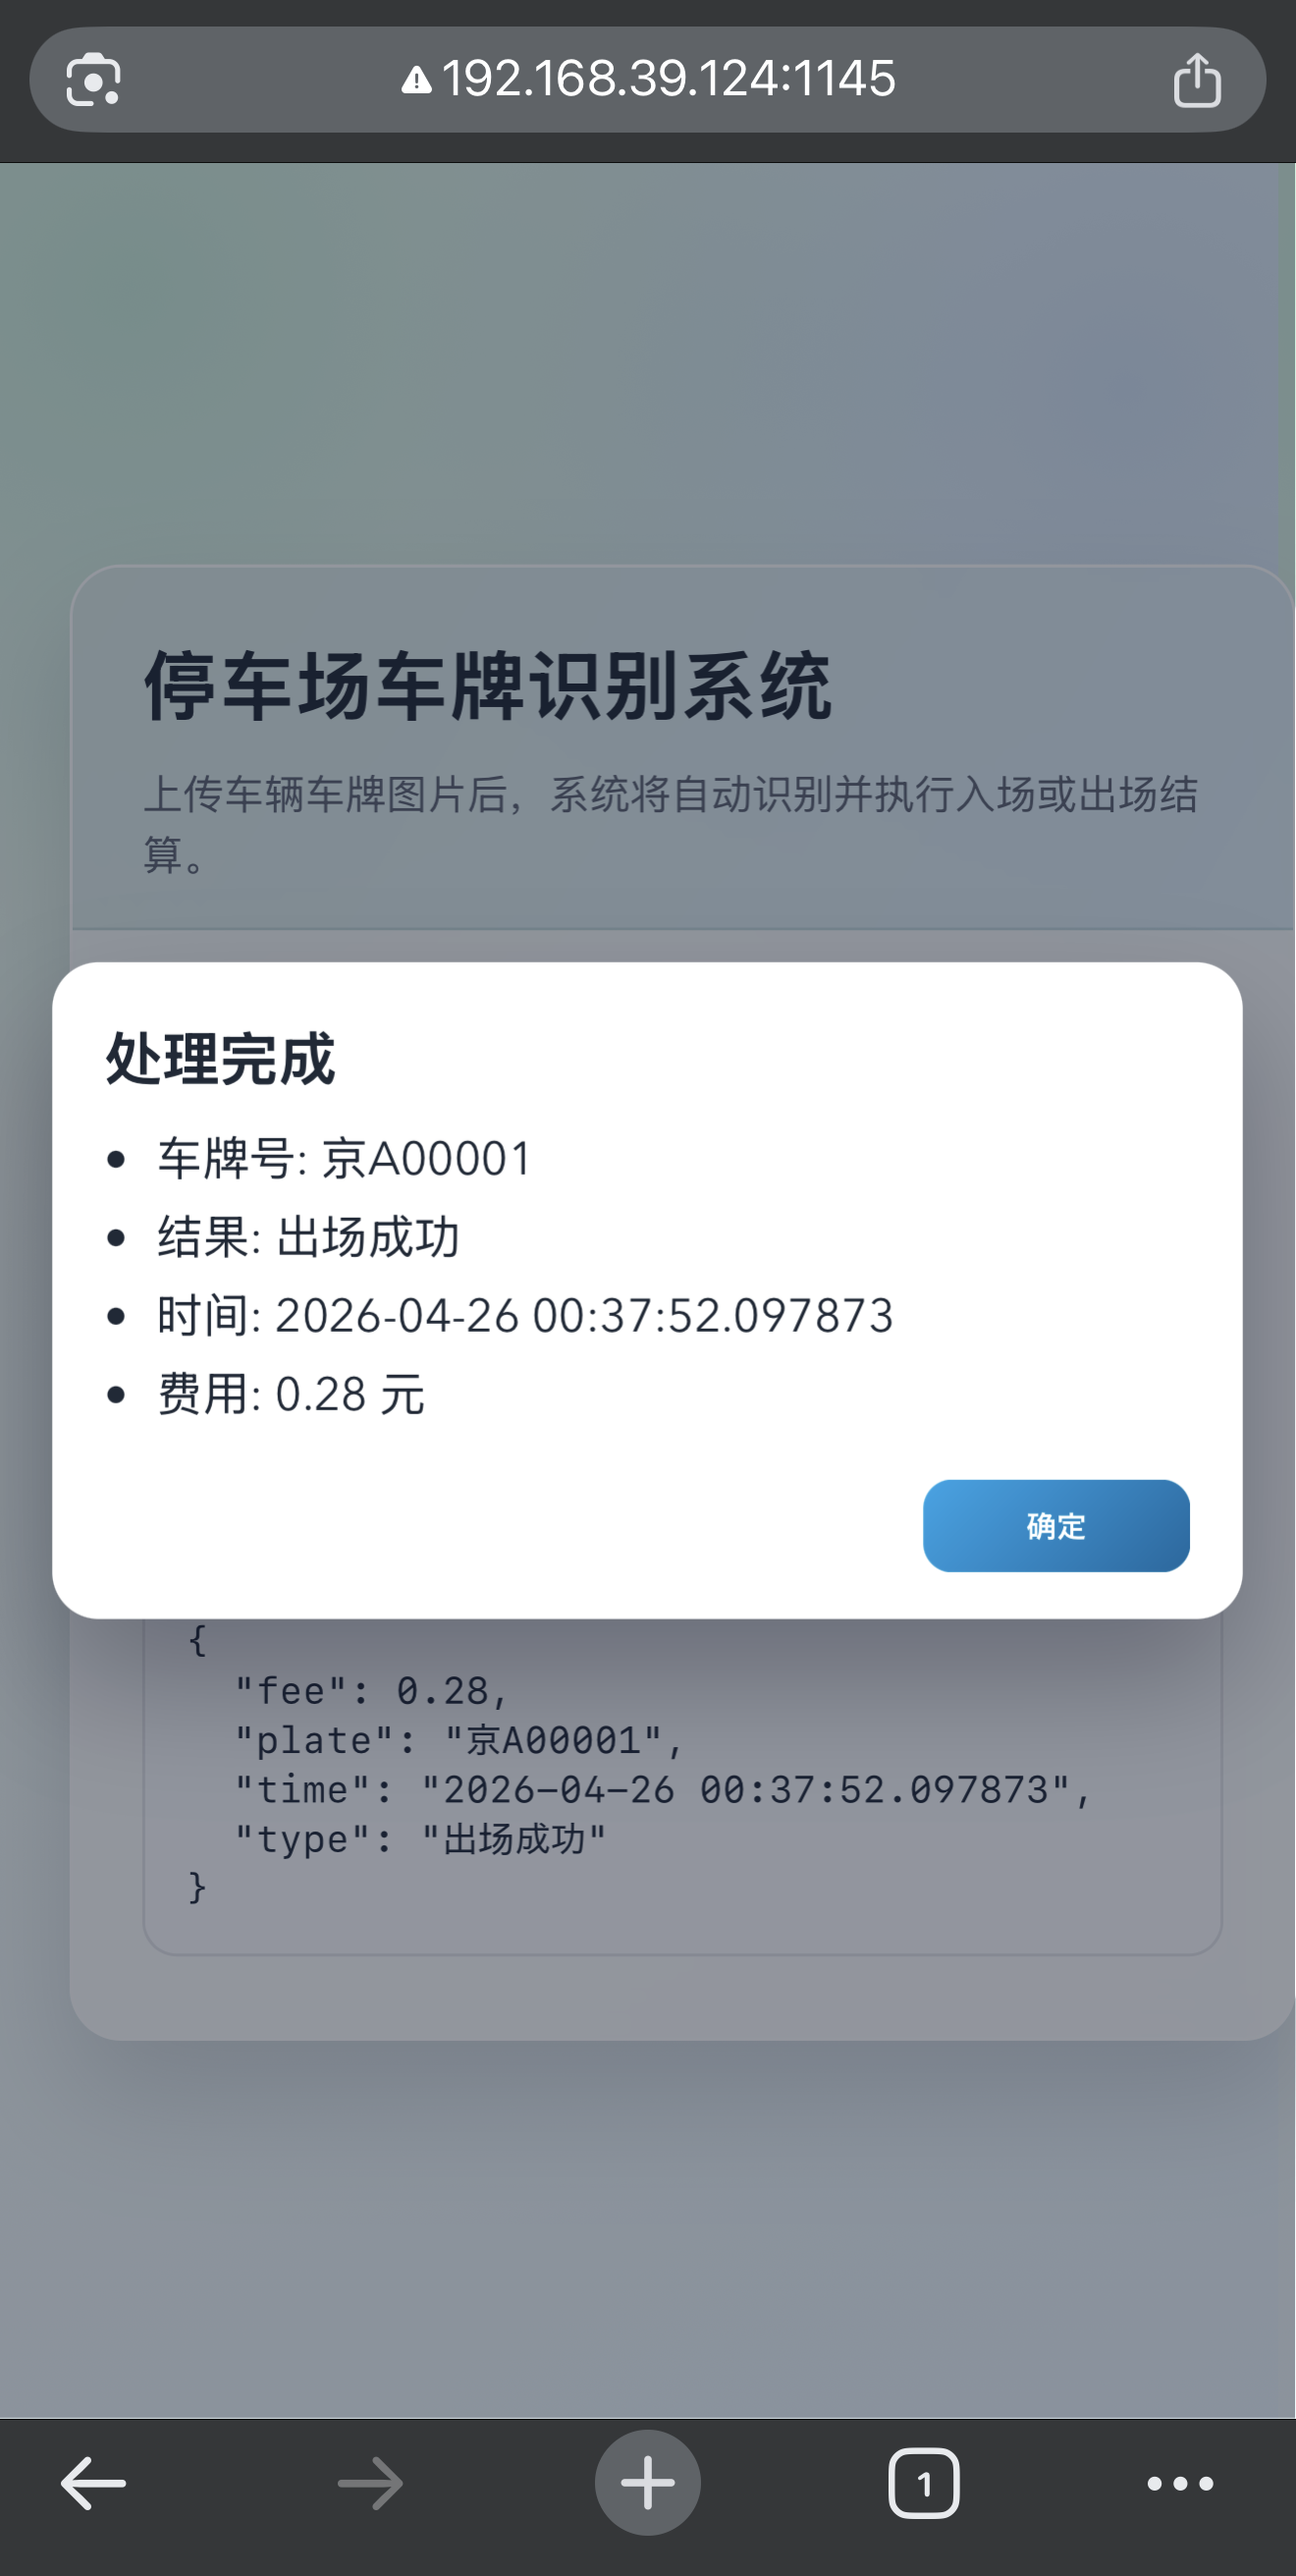
\includegraphics[width=0.44\textwidth]{images/test_3_exit_webui.png}
  \caption{测试三出场：前端弹窗结果（含费用）}
  \label{fig:t3-exit-ui}
\end{figure}

\textbf{分析：}测试三是最有代表性的复杂场景。图中可见系统并非“单次识别失败即终止”，而是依赖候选区域排序与逐个尝试策略，在第二候选成功匹配规则。这说明改进方案具有工程上的容错能力。

\subsection*{4. 综合结果分析}
综合三组测试共六次业务请求（每组入场+出场），系统均返回\texttt{200}并完成正确业务流转。结合日志分析，可得到以下结论：
\begin{enumerate}
  \item 候选区域定位显著降低整图背景干扰，尤其对高分辨率图像有明显收益。
  \item 规则过滤能有效抑制“可读但不合法”的OCR字符串，减少误入库风险。
  \item 城市位纠偏机制对\texttt{B/8}、\texttt{I/1}等混淆问题有实用价值。
  \item 颜色约束与后缀长度约束提升了结果可解释性：蓝牌5位尾号、绿牌6位尾号。
  \item 前端弹窗反馈与日志信息一致，用户可清晰感知系统状态。
\end{enumerate}

同时也观察到一个与平台相关但不影响正确性的提示：在Apple芯片MPS环境下，PyTorch会输出\texttt{pin\_memory}警告，该告警不影响识别结果，可在后续通过运行配置进一步优化。

\section*{七、实验结论}
本实验完成了一个可在局域网中运行的停车场车牌识别与计费系统，满足了“上传图片—识别车牌—自动判定入场/出场—返回结果与费用”的核心需求。与基础版本相比，规则增强版在鲁棒性和工程可用性方面均有明显提升：

\begin{itemize}
  \item 在识别策略上，实现了“颜色候选定位+两阶段OCR+规则融合”的完整管线；
  \item 在业务规则上，实现了符合中国车牌结构的硬约束，并支持蓝牌/绿牌差异化处理；
  \item 在系统工程上，实现了可追踪日志、错误状态码、移动端友好界面与弹窗反馈；
  \item 在测试结果上，三组样本入场出场流程均正确完成，说明系统闭环运行稳定。
\end{itemize}

在实验要求的加分项方向上，本系统已实现：车位管理（总车位/剩余车位维护与入场校验）、管理员后台（记录查看、费率与车位配置修改、收费报表CSV导出）、车牌识别缓存（同图免重复识别）、上传图片定期清理、文件日志模块以及多线程并发处理。

总体而言，本实验达到了预期教学目标，具备继续扩展为课程项目或小型演示系统的基础。

\section*{八、总结及心得体会}
通过本次实验，我们对“算法正确”与“系统可用”之间的差异有了更直观的理解。最初的想法是直接把图片送入OCR并取第一段文本，但在真实测试中很快暴露出多个问题：背景干扰、字符混淆、区域偏移、格式不一致等。这些问题说明，视觉识别在工程场景里往往不是单模型即可解决，而是需要“模型能力+先验知识+流程控制”共同作用。

在调试过程中，服务端日志发挥了决定性作用。我们通过观察每一次请求的候选区域数量、OCR原始输出、分区OCR结果、规则匹配路径，能够快速定位是“定位失败”“识别失败”还是“规则过严/过松”。例如城市位误识别的修正，就是基于日志发现“\texttt{8}频繁出现在城市位”这一现象后，有针对性加入映射和打分策略完成的。这个过程让我们认识到：可观测性是工程系统迭代的前提。

另外，前端交互细节同样影响整体体验。实验中如果只在控制台输出JSON，普通用户难以理解系统状态。加入弹窗、结果分行展示和确认按钮后，用户可以直观看到“车牌号、入/出场状态、时间、费用”，系统可用性明显提高。移动端测试也让我们意识到，课程项目不应只在PC端可用，良好的响应式布局是基本工程要求。

从知识融合角度看，本实验同时涉及网络编程、数据库、图像处理和规则系统，体现了跨模块协同的重要性。未来若继续优化，我们计划：
\begin{enumerate}
  \item 增加更丰富样本集，评估不同光照、角度、遮挡条件下的识别性能；
  \item 引入按车型、停车时段的差异化计费策略；
  \item 将开发服务器迁移到生产级WSGI部署（如Gunicorn），进一步增强并发处理能力；
  \item 在管理员后台基础上增加登录鉴权、按时间区间统计与图表化报表。
\end{enumerate}

总的来说，本实验不仅完成了功能实现，更重要的是建立了“问题发现—日志定位—规则修正—回归测试”的工程思维路径，这对后续课程设计与实际项目开发都具有长期价值。

\section*{附件}
\subsection*{1. 源码文件说明}
实验核心源码包括：
\begin{itemize}
  \item \texttt{app.py}：服务端主程序，包含OCR识别、规则过滤、识别缓存、车位管理、数据库读写、日志模块、上传清理与全部接口逻辑。
  \item \texttt{templates/index.html}：移动端页面，包含拍摄/相册取图、图片预览、入场/出场/智能通道、进度提示、结果弹窗与剩余车位展示。
  \item \texttt{templates/admin.html}：管理员后台页面，包含记录列表、车位/收入统计、费率配置与报表导出入口。
  \item \texttt{parking.db}：SQLite数据库文件（\texttt{cars}记录表与\texttt{config}配置表）。
  \item \texttt{server.log}：服务端滚动日志文件。
\end{itemize}

\subsection*{2. 关键附件嵌入示例（日志片段）}
\begin{lstlisting}
INFO ... Detected 2 plate region candidate(s)
INFO ... Plate-crop OCR (allowlist): ['8929121']
INFO ... ROI OCR province=['SU'], city=['8','8'], tail=['929121']
INFO ... Plate matched in region #1: SU-B92912
INFO ... Entry recorded: plate=SU-B92912, time=...
\end{lstlisting}

以上日志片段展示了“候选区域定位—分区OCR—规则纠偏—业务写库”的完整链路。

\end{document}